\documentclass[10pt]{article}

\usepackage[T1]{fontenc}
\usepackage[utf8]{inputenc}
\usepackage{mathptmx}
\usepackage[
  paperwidth=595.276pt,
  paperheight=793.701pt,
  left=37pt,
  right=37pt,
  top=34pt,
  bottom=43pt
]{geometry}
\usepackage[protrusion=true,expansion=false]{microtype}
\usepackage{amsmath,amssymb}
\usepackage{booktabs,tabularx,array,multirow}
\usepackage{graphicx}
\usepackage{xcolor}
\usepackage{caption}
\usepackage{subcaption}
\usepackage{enumitem}
\usepackage{fancyhdr}
\usepackage{hyperref}
\usepackage{tikz}
\usetikzlibrary{arrows.meta,positioning,calc}

\graphicspath{
  {../plots/}
  {../plots/extended_research/}
  {../plots/lifetime_modeling/}
  {../../results/cross_dataset_research/plots/}
  {../../results/vmd/}
  {../../results/modeling/}
  {../../results/interpretation/}
  {../../results/feature_selection/}
  {../../results/eda/}
}

\definecolor{sdblue}{HTML}{0076A8}
\definecolor{lightpanel}{HTML}{E8E8E8}
\definecolor{ink}{HTML}{1B1B1B}
\definecolor{muted}{HTML}{4F4F4F}
\definecolor{teal}{HTML}{147C7C}
\definecolor{amber}{HTML}{B66B00}
\definecolor{brick}{HTML}{A64032}
\definecolor{panel}{HTML}{F4F7F8}
\definecolor{linegray}{HTML}{CBD5DA}

\hypersetup{
  colorlinks=true,
  linkcolor=sdblue,
  citecolor=sdblue,
  urlcolor=sdblue,
  pdftitle={From Sensor Signatures to Survival Curves},
  pdfauthor={Amrit Lahari, Sukrit Agarwal, Pushkar Agrawal, Amit Kumar Jain},
  pdfsubject={Detailed research paper in Reliability Engineering and System Safety style}
}

\setlength{\columnsep}{20pt}
\setlength{\parindent}{9pt}
\setlength{\parskip}{0pt}
\setlength{\textfloatsep}{5pt plus 1pt minus 1pt}
\setlength{\floatsep}{4pt plus 1pt minus 1pt}
\setlength{\intextsep}{5pt plus 1pt minus 1pt}
\setlist[itemize]{leftmargin=1.1em,itemsep=0.1em,topsep=0.2em}
\setlist[enumerate]{leftmargin=1.25em,itemsep=0.1em,topsep=0.2em}
\captionsetup{font=footnotesize,labelfont=bf,skip=3pt}
\captionsetup[subfigure]{font=scriptsize,skip=2pt}
\renewcommand{\arraystretch}{1.08}
\raggedbottom
\emergencystretch=2em

\newcolumntype{Y}{>{\raggedright\arraybackslash}X}
\newcommand{\vb}{V\!B}
\newcommand{\vbtr}{V\!B_{\mathrm{tr}}}
\newcommand{\vbf}{V\!B_{\mathrm{f}}}
\newcommand{\earlyexp}{m_{\mathrm{e}}}
\newcommand{\lateexp}{m_{\mathrm{l}}}
\newcommand{\phii}{\phi}
\newcommand{\ttr}{t_{\mathrm{tr}}}
\newcommand{\dataset}[1]{\textsf{#1}}
\newcommand{\code}[1]{\texttt{#1}}
\newcommand{\modelname}{\textsc{Predict}}

\makeatletter
\renewcommand\section{\@startsection{section}{1}{0pt}%
  {1.15em plus .2em minus .1em}{0.55em}{\normalfont\normalsize\bfseries}}
\renewcommand\subsection{\@startsection{subsection}{2}{0pt}%
  {0.9em plus .15em minus .1em}{0.35em}{\normalfont\small\bfseries}}
\renewcommand\subsubsection{\@startsection{subsubsection}{3}{0pt}%
  {0.65em plus .1em minus .1em}{0.25em}{\normalfont\small\itshape}}
\makeatother

\pagestyle{fancy}
\fancyhf{}
\lhead{\footnotesize A. Lahari et al.}
\rhead{\footnotesize Reliability Engineering and System Safety-style format 2026}
\cfoot{\footnotesize\thepage}
\renewcommand{\headrulewidth}{0pt}
\setlength{\headheight}{13pt}

\newcommand{\journalheader}{%
  \noindent\rule{\textwidth}{0.55pt}
  \vspace{0.55em}
  \noindent
  \begin{minipage}[c]{0.13\textwidth}
    \centering
    {\Large\bfseries E}\\[-0.1em]
    {\scriptsize ELSEVIER}\\[-0.2em]
    \rule{0.78\linewidth}{0.35pt}
  \end{minipage}\hfill
  \begin{minipage}[c]{0.72\textwidth}
    \centering
    \colorbox{lightpanel}{%
      \begin{minipage}{0.95\linewidth}
        \centering
        \vspace{0.35em}
        {\small Contents lists available at \textcolor{sdblue}{ScienceDirect}}\par
        \vspace{0.9em}
        {\LARGE Reliability Engineering and System Safety}\par
        \vspace{0.75em}
        {\small journal homepage: \textcolor{sdblue}{www.elsevier.com/locate/ress}}
        \vspace{0.35em}
      \end{minipage}}
  \end{minipage}\hfill
  \begin{minipage}[c]{0.10\textwidth}
    \centering
    \fbox{\begin{minipage}{0.78\linewidth}
      \centering
      \tiny RELIABILITY\\ENGINEERING\\\& SYSTEM\\SAFETY
    \end{minipage}}
  \end{minipage}
  \vspace{0.55em}
  \noindent\rule{\textwidth}{0.55pt}
  \vspace{2.2em}
}

\begin{document}
\thispagestyle{empty}
\twocolumn[{
\begin{@twocolumnfalse}
\journalheader

{\LARGE From sensor signatures to survival curves: a physics-regularized digital twin for milling tool wear and tool-life forecasting\par}
\vspace{0.75em}
{\large Amrit Lahari\textsuperscript{a}, Sukrit Agarwal\textsuperscript{a}, Pushkar Agrawal\textsuperscript{a}, Amit Kumar Jain\textsuperscript{a,*}\par}
\vspace{0.35em}
{\footnotesize
\textsuperscript{a}Department of Mechanical Engineering, Birla Institute of Technology and Science, Pilani, India\par
\textsuperscript{*}Corresponding supervisor.
\par}
\vspace{2.45em}

\noindent
\begin{minipage}[t]{0.26\textwidth}
  {\footnotesize A R T I C L E \ \ I N F O}\par
  \vspace{0.8em}
  \rule{\linewidth}{0.55pt}\par
  \vspace{0.45em}
  {\footnotesize\itshape Keywords:}\par
  {\footnotesize
  Milling tool wear\par
  Tool-life forecasting\par
  Remaining useful life\par
  Physics-regularized regression\par
  Variational mode decomposition\par
  Accelerated failure time\par
  Digital twin\par}
\end{minipage}
\hfill
\begin{minipage}[t]{0.68\textwidth}
  {\footnotesize A B S T R A C T}\par
  \vspace{0.8em}
  \rule{\linewidth}{0.55pt}\par
  \vspace{0.45em}
  {\footnotesize
  This paper reports the integrated research workflow developed for milling tool wear and tool-life forecasting. The work begins with NASA milling exploratory analysis, feature extraction and leave-one-case-out wear modeling, expands to cross-dataset health baselines, and then connects those empirical signals to physics-regularized lifetime estimation. Three complementary public milling sources are used: \dataset{NUAA}/\dataset{UniWear} orthogonal milling records for process-load effects, \dataset{PHM2010} cutter trajectories for early-regime transfer, and \dataset{NASA} milling run-to-failure data for late-stage acceleration, sensor evidence and material effects. The central objective is not only to minimize pointwise wear error, but to construct an interpretable, simulator-ready model that links process variables, sensor signatures, uncertainty and threshold-crossing life. The proposed framework combines (i) dataset-role analysis, (ii) grouped validation for wear regression and failure classification, (iii) time-domain, FFT and variational-mode-decomposition features, (iv) a physics-regularized piecewise wear law with early exponent \(\earlyexp=0.64\) and late exponent \(\lateexp=1.29\), (v) bootstrap intervals and residual diagnostics, and (vi) lifetime extraction by training wear models and inverting them into crossing times. Feed emerges as the most reliable local load driver. VMD improves the strongest absolute feature-wear correlation from \(0.4806\) to \(0.5607\). The best pointwise wear regressor, Gradient Boosting, does not give the best event-life forecast after inversion, showing that optimizing wear RMSE is not equivalent to optimizing tool-life prediction. The resulting digital-twin prototype is suitable for research simulation, scenario ranking and explanation, but requires larger full-life validation before industrial deployment.}
\end{minipage}

\vspace{1.8em}
\noindent\rule{\textwidth}{0.55pt}
\vspace{1.0em}
\end{@twocolumnfalse}
}]

\section{Introduction}

Milling tool wear is not a single regression problem. A cutting edge can spend a long interval in slow early wear, then move into accelerated damage where a small amount of additional cutting time produces a large increase in flank wear. A realistic monitoring system therefore has to answer four coupled questions. First, it must describe the physical progression from early wear to accelerated wear. Second, it must explain how spindle speed, feed and depth alter the rate of that progression. Third, it must identify which vibration, acoustic-emission or current signatures provide evidence that the tool is moving toward failure. Fourth, it must translate a trained wear model into a practical replacement-time or remaining-useful-life estimate.

The project reported here was built around those questions. The workflow starts with NASA milling exploratory analysis, hand-crafted time and frequency features, leave-one-case-out wear modeling, feature selection and interpretation. It then expands from one dataset to cross-dataset health baselines for PHM2010, NASA and UniWear, fits a physics-regularized piecewise wear equation, adds uncertainty intervals, calibration checks and residual diagnostics, and finally trains wear models that are inverted into threshold-crossing estimates and compared against accelerated-failure-time equations. This matters because a model that predicts flank wear well at individual samples is not necessarily a model that predicts the crossing time accurately.

The main contributions are as follows. A NASA sensor-modeling benchmark establishes the limits of raw feature regression under case-held-out validation. A dataset-role framework separates early-wear load evidence, early-exponent transfer evidence and late-stage acceleration evidence instead of pooling heterogeneous data blindly. A compact piecewise wear law explains why a single exponent is not enough. A cross-dataset health pipeline evaluates regression and failure classification under grouped validation. A VMD-based feature pass shows that modal features can improve wear correlation over raw signal descriptors. A lifetime-model extraction pipeline trains multiple wear models, inverts them into crossing estimates and exposes the mismatch between wear RMSE and life accuracy. Finally, bootstrap uncertainty, residual diagnostics and early-window calibration tests describe where the present digital twin is stable and where it remains under-identified.

\begin{figure*}[!t]
  \centering
  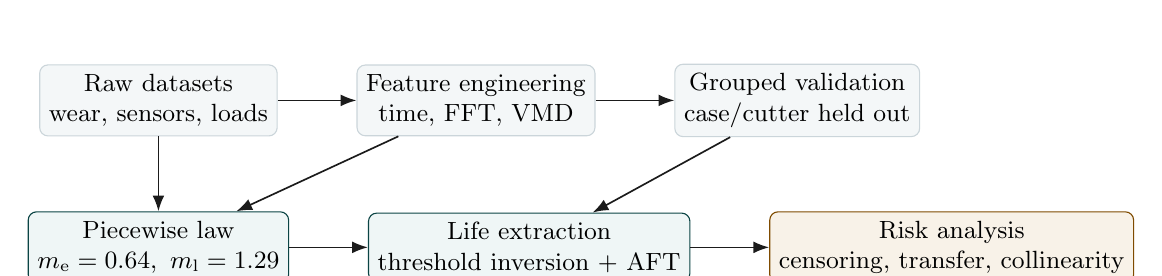
\begin{tikzpicture}[node distance=0.95cm and 1.0cm]
    \tikzset{
      block/.style={rounded corners=3pt,draw=linegray,fill=panel,minimum width=3.0cm,minimum height=0.85cm,align=center,font=\small},
      result/.style={rounded corners=3pt,draw=teal!55!black,fill=teal!7,minimum width=3.0cm,minimum height=0.85cm,align=center,font=\small},
      warn/.style={rounded corners=3pt,draw=amber!70!black,fill=amber!9,minimum width=3.0cm,minimum height=0.85cm,align=center,font=\small},
      arrow/.style={-{Latex[length=2mm]},draw=ink,line width=0.6pt}
    }
    \node[block] (raw) {Raw datasets\\wear, sensors, loads};
    \node[block,right=of raw] (feat) {Feature engineering\\time, FFT, VMD};
    \node[block,right=of feat] (cv) {Grouped validation\\case/cutter held out};
    \node[result,below=of raw] (law) {Piecewise law\\\(\earlyexp=0.64,\ \lateexp=1.29\)};
    \node[result,right=of law] (life) {Life extraction\\threshold inversion + AFT};
    \node[warn,right=of life] (limits) {Risk analysis\\censoring, transfer, collinearity};
    \draw[arrow] (raw) -- (feat);
    \draw[arrow] (feat) -- (cv);
    \draw[arrow] (raw) -- (law);
    \draw[arrow] (feat) -- (law);
    \draw[arrow] (law) -- (life);
    \draw[arrow] (cv) -- (life);
    \draw[arrow] (life) -- (limits);
  \end{tikzpicture}
  \caption{Research architecture followed in the project. The workflow separates signal evidence, physics-regularized equation building, grouped validation, lifetime inversion and risk interpretation.}
  \label{fig:research-architecture}
\end{figure*}

\section{Background and research gap}

Tool condition monitoring literature has traditionally emphasized two tasks: estimating the current wear state from sensor signals and classifying a tool as healthy or faulty. Those tasks are important, but they are incomplete for replacement planning. A factory decision is a time-to-event decision: when is the tool likely to cross a failure threshold, and how much uncertainty surrounds that crossing time?

Survival analysis is useful because tool-life data often contain censoring. A cutter may not reach the selected wear threshold before the experiment ends. Treating that record as an ordinary non-failure discards information and biases the fitted life model. Accelerated-failure-time modeling gives a compact way to express how process variables multiply or compress expected lifetime. The project uses this idea directly for NUAA and NASA life equations.

Physics-informed learning is also necessary because public milling datasets are heterogeneous. Some sources contain many process settings but do not run all tools to severe failure. Others contain rich run-to-failure trajectories but fewer process variables. A single black-box regression over all records would conflate early and late wear physics, sensor differences, units and thresholds. The research gap addressed here is therefore not simply ``train a better regressor.'' The gap is to connect sparse experimental evidence, physics-guided structure, sensor features, uncertainty and threshold-crossing life in a single research-grade workflow.

\section{Data and evidence structure}

\subsection{Dataset roles}

Three datasets form the core evidence base, but they are not interchangeable. NUAA/UniWear carries the process variation needed to fit the load law. PHM2010 checks whether the early exponent transfers beyond one source. NASA provides severe wear progression, material effects and multi-sensor evidence. Table~\ref{tab:dataset-roles} summarizes these roles.

\begin{table*}[!t]
  \centering
  \caption{Primary datasets and their research roles.}
  \label{tab:dataset-roles}
  \footnotesize
  \begin{tabularx}{\textwidth}{p{2.6cm}p{3.0cm}p{3.2cm}Y}
    \toprule
    Dataset & Local role & Main measurements & Why it matters \\
    \midrule
    NUAA / UniWear & Early wear and process-condition law & Wear, spindle speed, feed per tooth, axial depth & Supplies process variation needed to fit the load-intensity function and lifetime surfaces. It includes censored runs, making survival-aware modeling necessary. \\
    PHM2010 & Early-regime transfer check & Cutter wear trajectories and derived features & Tests whether the early exponent learned from NUAA is a local artifact or a transferable early-wear slope. \\
    NASA Milling & Late-stage acceleration and material behavior & Vibration, acoustic emission, spindle current, wear, feed, depth, material & Contains severe wear progression and rich sensors, making it the best local source for accelerated wear, frequency-domain evidence and material-aware survival behavior. \\
    \bottomrule
  \end{tabularx}
\end{table*}

The failure thresholds are dataset-specific because the measurement scale and experimental intent differ. These thresholds are operational labels for local model comparison, not universal industrial replacement limits. PHM2010 uses \(0.150~\mathrm{mm}\), NASA uses \(0.300~\mathrm{mm}\) and UniWear uses \(0.220~\mathrm{mm}\). The corresponding failure rates are 0.1725, 0.4795 and 0.2743 respectively.

\begin{figure*}[!t]
  \centering
  \begin{minipage}[t]{0.37\textwidth}
    \vspace{0pt}
    \centering
    \captionof{table}{Dataset-specific health labels.}
    \label{tab:failure-thresholds}
    \scriptsize
    \setlength{\tabcolsep}{4pt}
    \renewcommand{\arraystretch}{1.15}
    \begin{tabularx}{\linewidth}{@{}lrrr@{}}
      \toprule
      Dataset & Samples & Threshold & Failure rate \\
      \midrule
      PHM2010 & 945 & \(0.150~\mathrm{mm}\) & 0.1725 \\
      NASA & 146 & \(0.300~\mathrm{mm}\) & 0.4795 \\
      UniWear & 649 & \(0.220~\mathrm{mm}\) & 0.2743 \\
      \bottomrule
    \end{tabularx}
    \vspace{0.55em}
    {\scriptsize
    \textbf{Derived threshold-label counts.}\par\vspace{0.15em}
    \setlength{\tabcolsep}{4pt}
    \renewcommand{\arraystretch}{1.08}
    \begin{tabularx}{\linewidth}{@{}lrr@{}}
      \toprule
      Dataset & Failed & Non-failed \\
      \midrule
      PHM2010 & 163 & 782 \\
      NASA & 70 & 76 \\
      UniWear & 178 & 471 \\
      \bottomrule
    \end{tabularx}
    \par\vspace{0.15em}
    \raggedright\emph{Check:} \(163/945=0.1725\), \(70/146=0.4795\) and \(178/649=0.2743\). Counts are derived from the sample totals and rounded failure rates above.\par}
  \end{minipage}
  \hfill
  \begin{minipage}[t]{0.59\textwidth}
    \vspace{0pt}
    \centering
    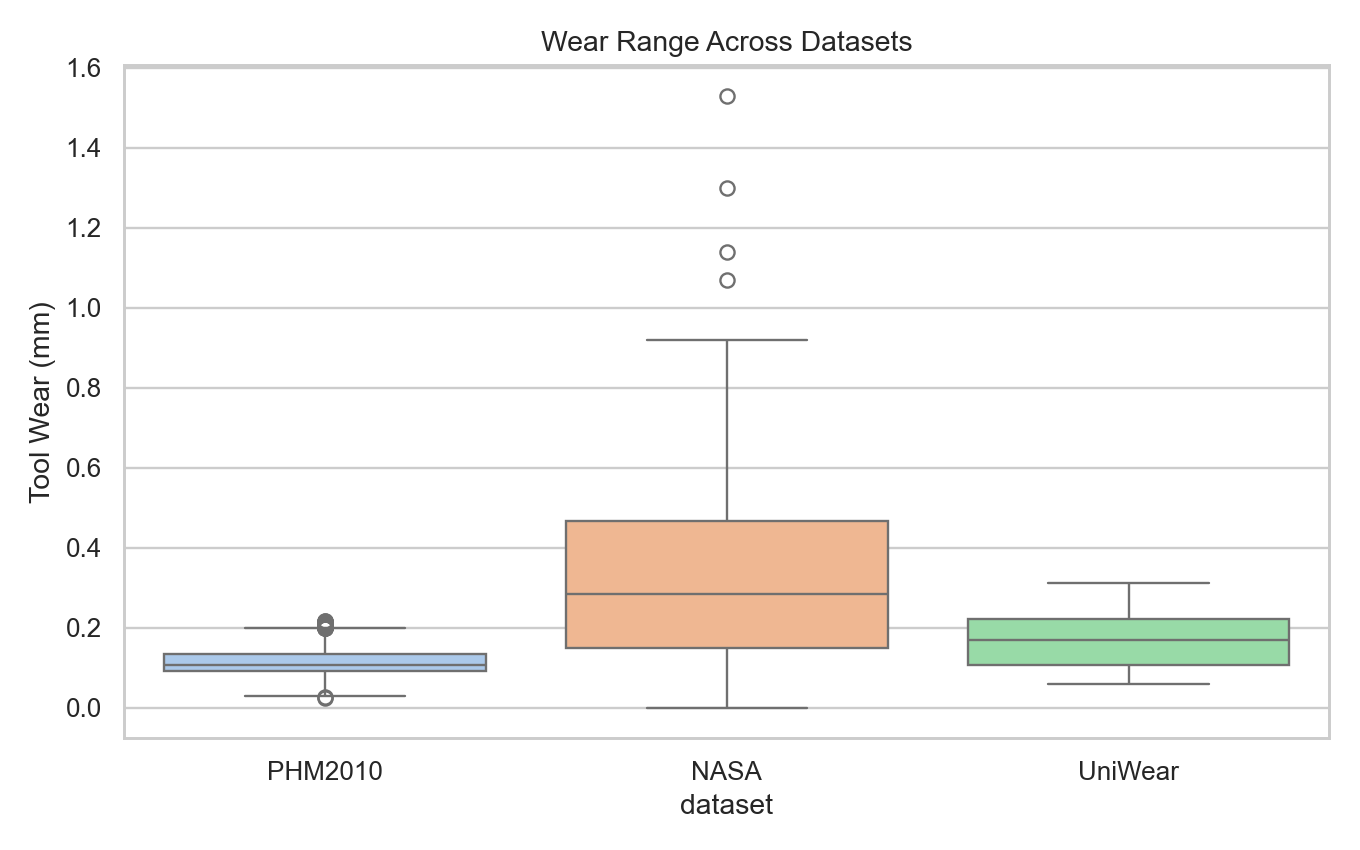
\includegraphics[width=\linewidth,height=0.23\textheight,keepaspectratio]{dataset_wear_distribution.png}
    \caption{Wear distributions across local datasets. Different ranges motivate dataset-specific thresholds and role-specific modeling.}
    \label{fig:wear-distribution}
  \end{minipage}
\end{figure*}

\subsection{Feature families}

The feature pipeline extracts compact descriptors from time-domain and frequency-domain signals. Time-domain level features include mean, root-mean-square and absolute mean. Shape features include skewness, kurtosis, crest factor and quantiles. Frequency features include FFT energy, dominant FFT bin, centroid and entropy. Process variables such as speed, feed, depth and material anchor the statistical features in machining physics.

\begin{table*}[!t]
  \centering
  \caption{Feature families and interpretation.}
  \label{tab:feature-families}
  \footnotesize
  \begin{tabularx}{\textwidth}{p{2.7cm}p{4.2cm}Y}
    \toprule
    Family & Examples & Tool-wear interpretation \\
    \midrule
    Time-domain level & mean, RMS, absolute mean & Captures load and energy growth as cutting becomes less efficient. \\
    Time-domain shape & skewness, kurtosis, crest factor, quantiles & Captures impulsive events, chatter bursts, rubbing and intermittent edge damage. \\
    Frequency-domain energy & FFT energy, peak bin, centroid, entropy & Captures shifts in vibration and acoustic-emission structure as wear changes cutting dynamics. \\
    VMD mode features & mode energy, entropy, center frequency, mode kurtosis & Separates mixed sensor signals into interpretable bands, improving some wear correlations over raw features. \\
    Process variables & speed, feed, axial depth, material & Enable scenario simulation and prevent the model from becoming purely sensor-specific. \\
    \bottomrule
  \end{tabularx}
\end{table*}

\subsection{Variational mode decomposition}

The NASA signal pass applies variational mode decomposition to vibration, acoustic emission and spindle-current channels. The settings are \(K=5\), \(\alpha=2000\) and \(\tau=0\). The pass produces 390 modal features over \code{vib\_spindle}, \code{vib\_table}, \code{AE\_table}, \code{AE\_spindle}, \code{smcAC} and \code{smcDC}. The strongest raw feature correlation with wear is \(|r|=0.4806\), while the strongest VMD feature reaches \(|r|=0.5607\). This is a 16.7\% improvement in the best absolute correlation.

\begin{figure*}[!t]
  \centering
  \begin{subfigure}[t]{0.49\textwidth}
    \centering
    \includegraphics[width=\textwidth]{vmd_vs_raw_comparison.png}
    \caption{Raw versus VMD correlation}
  \end{subfigure}
  \hfill
  \begin{subfigure}[t]{0.49\textwidth}
    \centering
    \includegraphics[width=\textwidth]{vmd_mode_spectra.png}
    \caption{Mode spectra}
  \end{subfigure}
  \caption{VMD separates broadband machining signals into mode-specific frequency content before feature extraction.}
  \label{fig:vmd-summary}
\end{figure*}

\begin{table*}[!t]
  \centering
  \caption{Top VMD features by absolute correlation with NASA flank wear.}
  \label{tab:top-vmd-features}
  \footnotesize
  \begin{tabularx}{\textwidth}{p{4.8cm}rrY}
    \toprule
    Feature & \(r\) & \(|r|\) & Interpretation \\
    \midrule
    \code{vib\_spindle\_m3\_skewness} & 0.5607 & 0.5607 & Wear increases asymmetric spindle vibration bursts. \\
    \code{smcDC\_m5\_entropy} & -0.5604 & 0.5604 & Current structure becomes less evenly distributed in the high-order mode. \\
    \code{vib\_spindle\_m5\_kurtosis} & 0.5542 & 0.5542 & Impulsive high-frequency vibration grows with tool damage. \\
    \code{vib\_table\_m4\_center\_freq} & -0.5287 & 0.5287 & Table vibration frequency content shifts as cutting stiffness changes. \\
    \code{vib\_spindle\_m1\_skewness} & 0.5079 & 0.5079 & Low-mode spindle asymmetry tracks progressive wear. \\
    \bottomrule
  \end{tabularx}
\end{table*}

Feature selection and SHAP analysis support the same conclusion: useful predictors are not only raw amplitude measures. Wear information appears in modal center frequency, entropy, kurtosis and acoustic-emission frequency terms. This is important for the simulator because it gives a richer evidence layer than simply measuring one RMS channel.

\begin{figure}[!htbp]
  \centering
  \includegraphics[width=\columnwidth]{shap_summary.png}
  \caption{SHAP summary for the NASA modeling pass. High-impact predictors include VMD center-frequency, entropy and kurtosis terms.}
  \label{fig:shap-summary}
\end{figure}

\section{Physics-regularized wear model}

\subsection{Rationale}

The piecewise law is the central modeling choice. A single power-law fit forces early and late wear into one compromise exponent. That is unsuitable for tool-life forecasting because the replacement decision is dominated by behavior near the threshold. The project therefore separates the early sub-linear regime from the accelerated late regime while keeping the equation compact enough for simulator use.

The model uses a reference-point process-load function \(\phii(n,f_z,a_p)\) and regime-specific exponents:

\begin{equation}
\vb(t)=
\begin{cases}
k_{\mathrm{e}}\phii(n,f_z,a_p)t^{\earlyexp}, & t \leq \ttr,\\
\vbtr+k_{\mathrm{l}}(t-\ttr)^{\lateexp}, & t>\ttr.
\end{cases}
\label{eq:piecewise}
\end{equation}

The transition value is
\begin{equation}
\vbtr=k_{\mathrm{e}}\phii(n,f_z,a_p)\ttr^{\earlyexp},
\label{eq:transition}
\end{equation}
and the early condition intensity is
\begin{equation}
\phii=
\left(\frac{n}{1800}\right)^{0.359967}
\left(\frac{f_z}{0.05}\right)^{3.956013}
\left(\frac{a_p}{3.0}\right)^{0.688073}.
\label{eq:condition-intensity}
\end{equation}

The estimated early law is
\begin{equation}
\vb(t)=0.018580943\,\phii\,t^{0.64}.
\label{eq:early-law}
\end{equation}

\subsection{Evidence for the exponents}

The exponent values are not fitted from one pooled curve. NUAA is used for the load-dependent early law, PHM2010 checks early-regime transfer and NASA provides late acceleration. The resulting evidence is summarized in Table~\ref{tab:exponent-evidence}.

\begin{table}[!htbp]
  \centering
  \caption{Evidence used to select the piecewise wear exponents.}
  \label{tab:exponent-evidence}
  \scriptsize
  \begin{tabularx}{\columnwidth}{p{1.3cm}p{1.1cm}rrY}
    \toprule
    Dataset & Regime & Exp. & RMSE & Role \\
    \midrule
    NUAA & Early & 0.6347 & 0.0211 & Main sub-linear early law. \\
    PHM2010 & Early & 0.6471 & 0.0136 & Transfer check. \\
    NASA & Late & 1.2873 & 0.0438 & Accelerated late behavior. \\
    \bottomrule
  \end{tabularx}
\end{table}

\begin{figure*}[!t]
  \centering
  \begin{subfigure}[t]{0.32\textwidth}
    \centering
    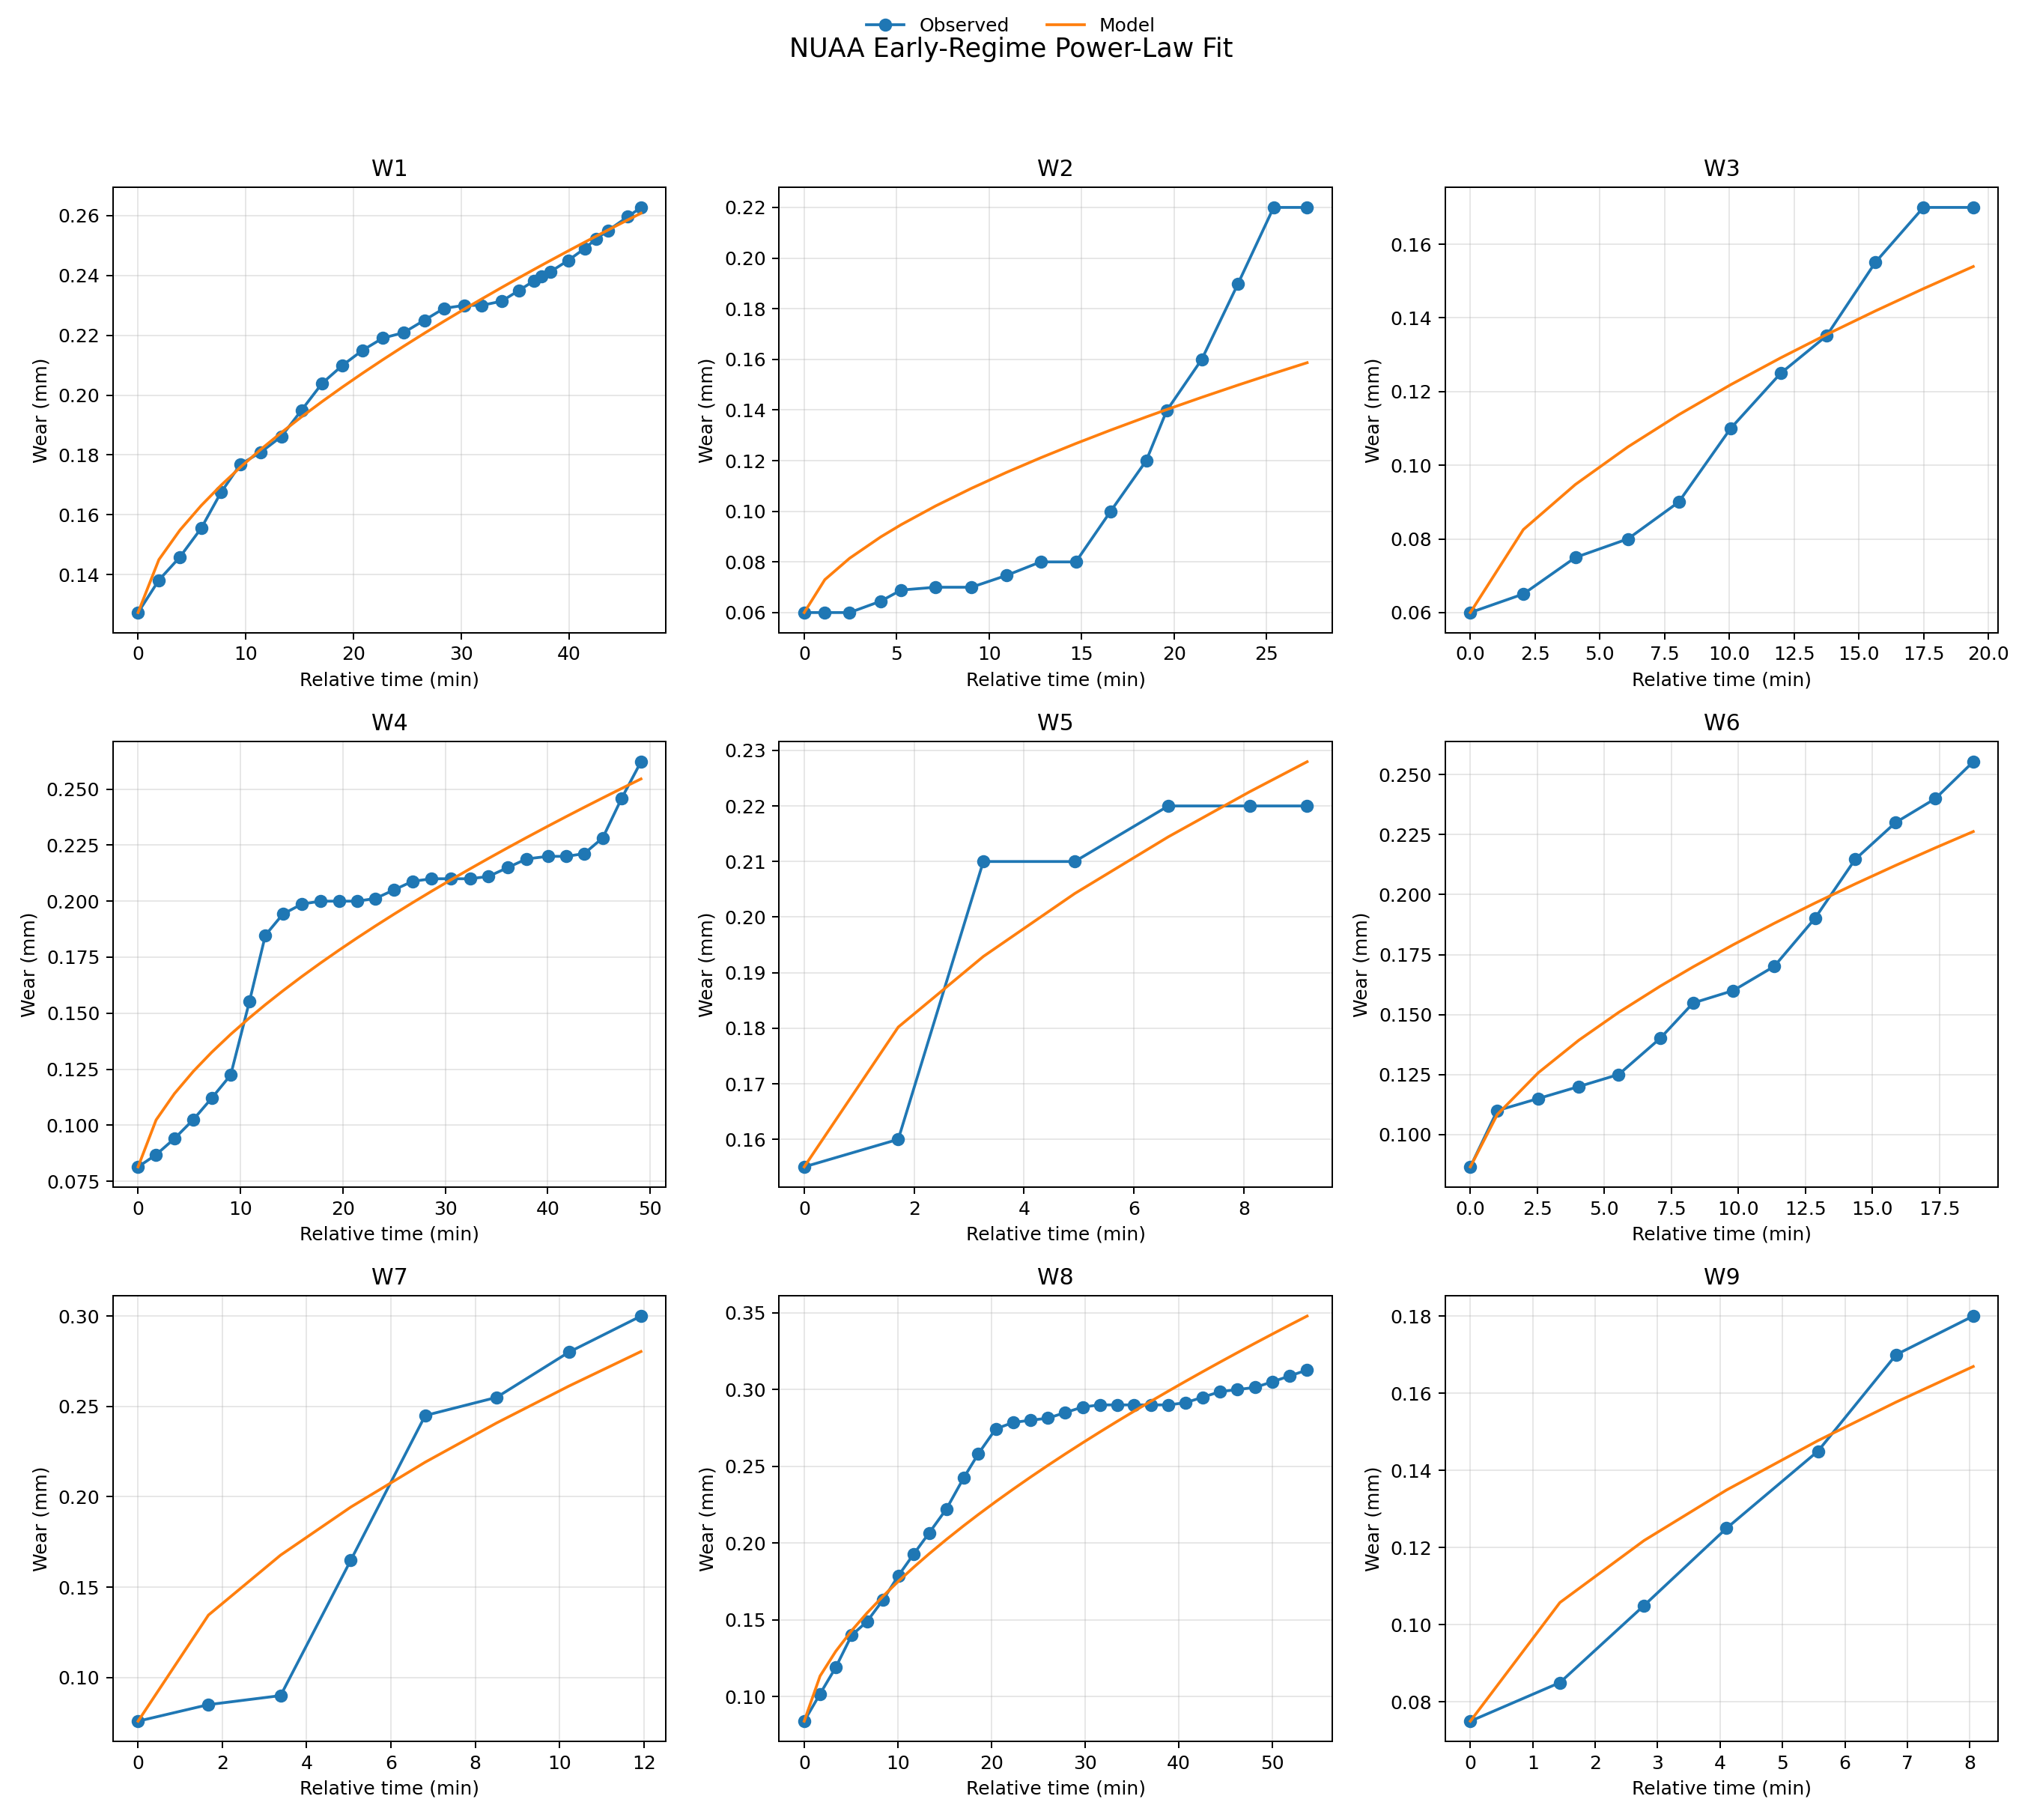
\includegraphics[width=\textwidth,height=0.24\textheight,keepaspectratio]{nuaa_early_regime_fit.png}
    \caption{NUAA early fit}
  \end{subfigure}
  \hfill
  \begin{subfigure}[t]{0.32\textwidth}
    \centering
    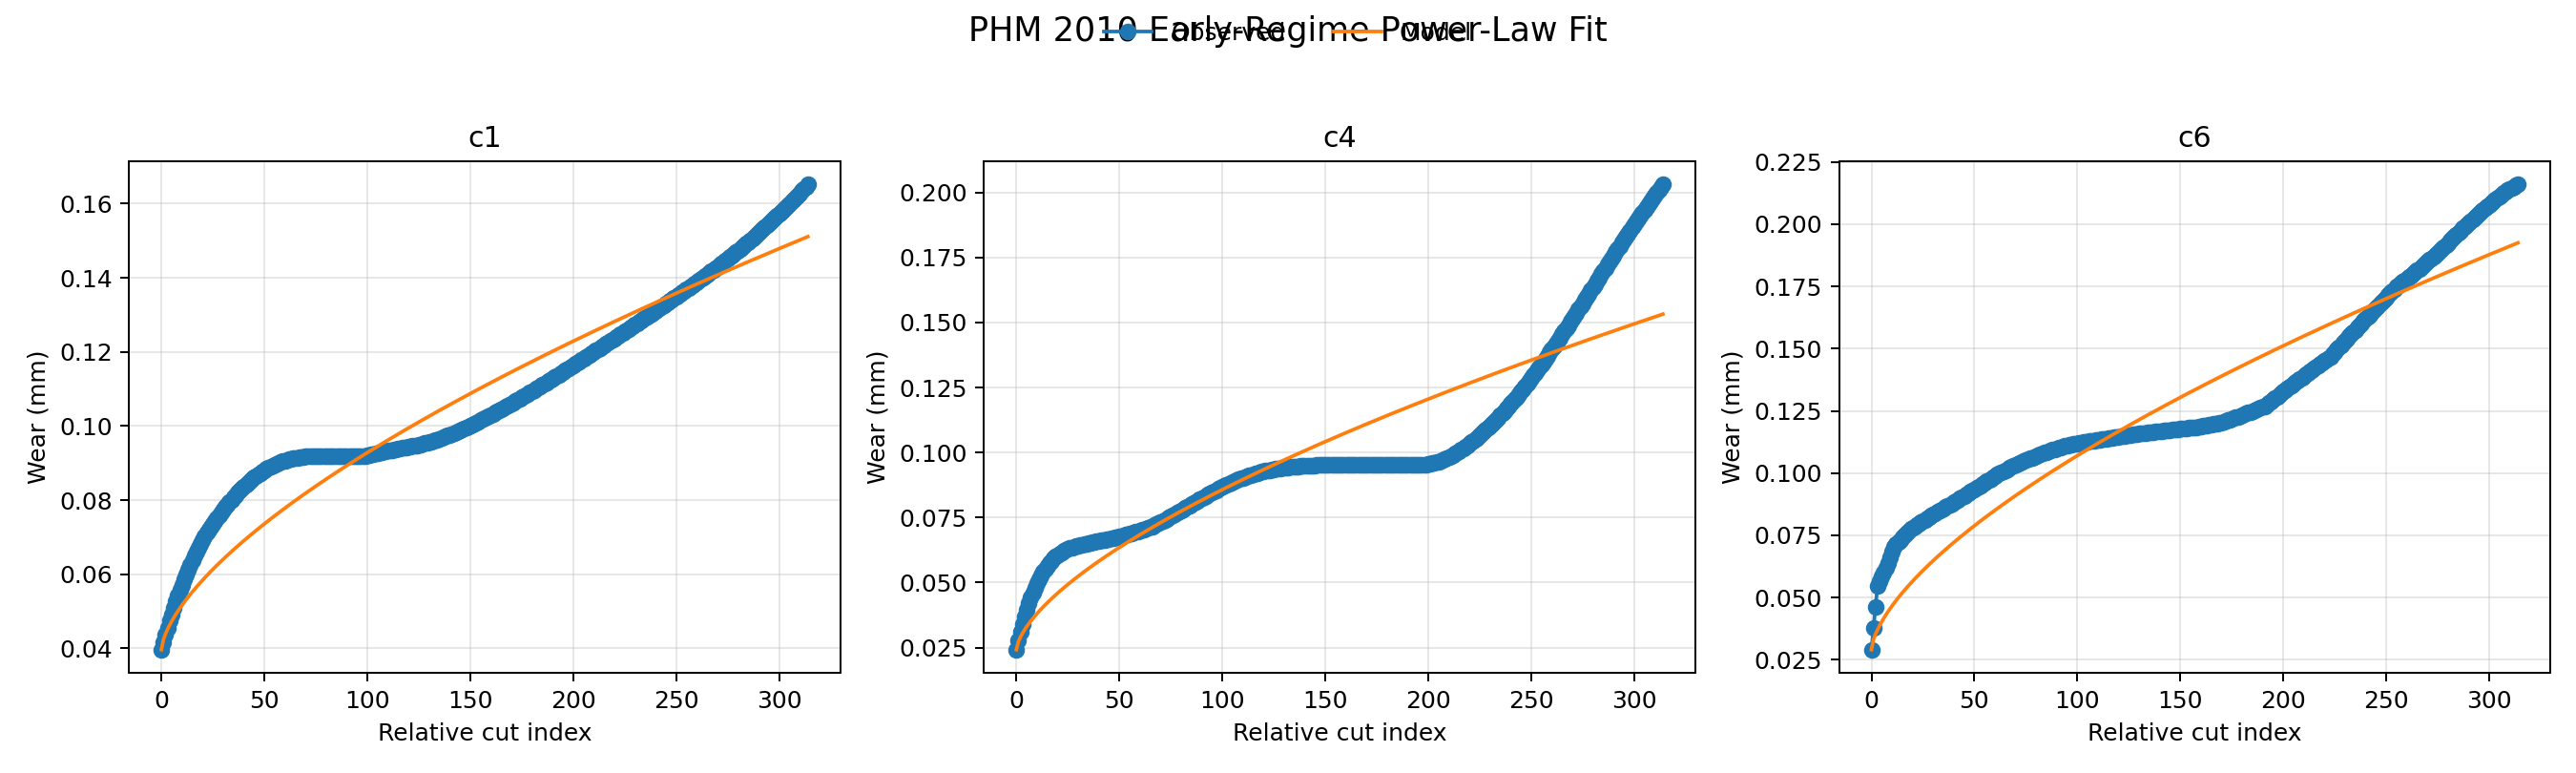
\includegraphics[width=\textwidth,height=0.24\textheight,keepaspectratio]{phm_early_regime_fit.png}
    \caption{PHM2010 transfer}
  \end{subfigure}
  \hfill
  \begin{subfigure}[t]{0.32\textwidth}
    \centering
    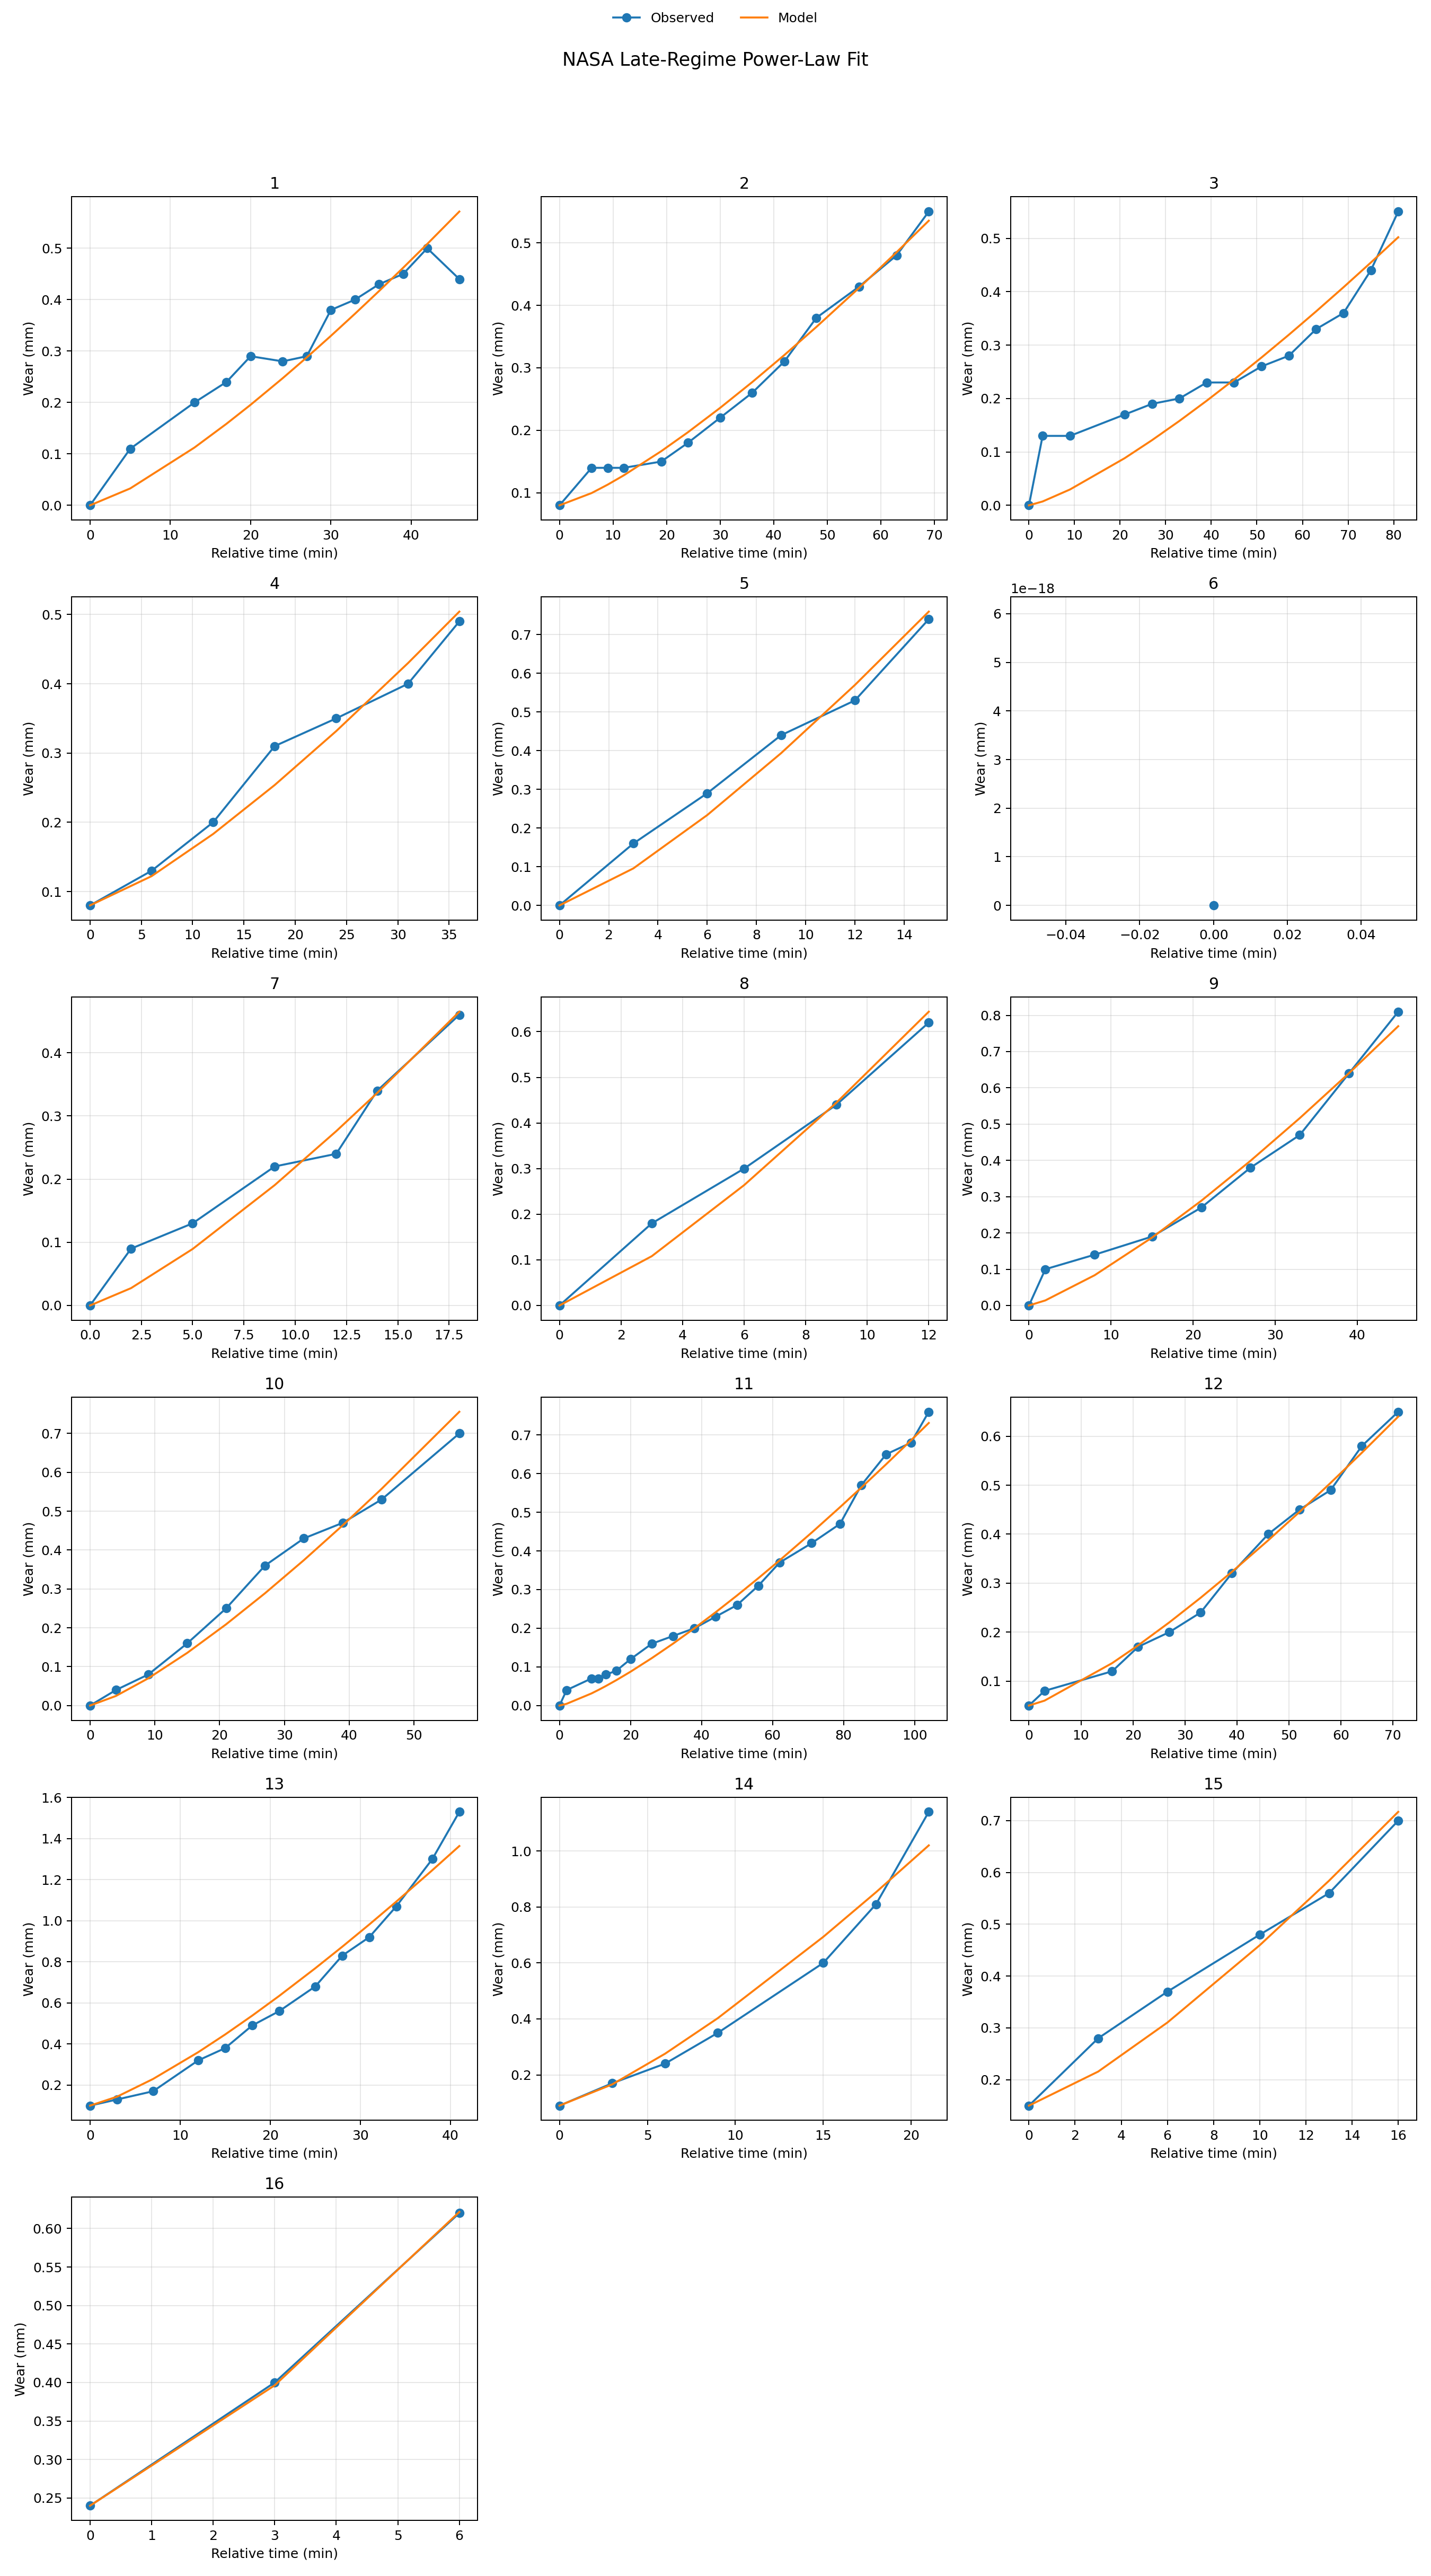
\includegraphics[width=\textwidth,height=0.24\textheight,keepaspectratio]{nasa_late_regime_fit.png}
    \caption{NASA late fit}
  \end{subfigure}
  \caption{Role-specific fits used to ground the early and late exponents.}
  \label{fig:regime-fits}
\end{figure*}

The fitted condition law is strongest in feed. This result is physically plausible because feed directly changes chip thickness and cutting load per tooth. Speed and depth also matter, but in the local NUAA design the feed exponent is more stable and much larger than the others. Bootstrap diagnostics later confirm that feed is the most consistently identified process variable in this design.

\begin{figure*}[!t]
  \centering
  \begin{subfigure}[t]{0.49\textwidth}
    \centering
    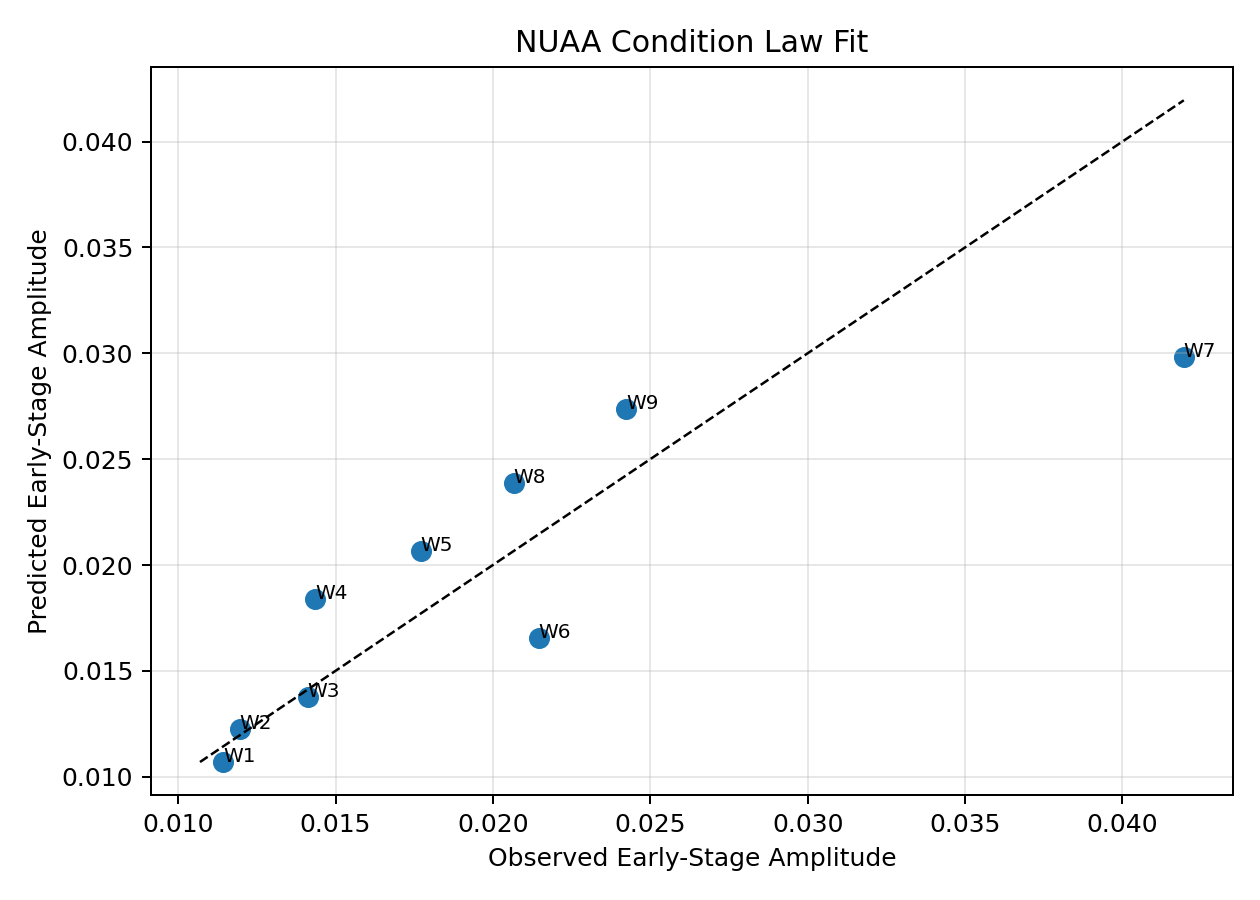
\includegraphics[width=\textwidth,height=0.22\textheight,keepaspectratio]{nuaa_condition_law_fit.png}
    \caption{Condition-law fit}
  \end{subfigure}
  \hfill
  \begin{subfigure}[t]{0.49\textwidth}
    \centering
    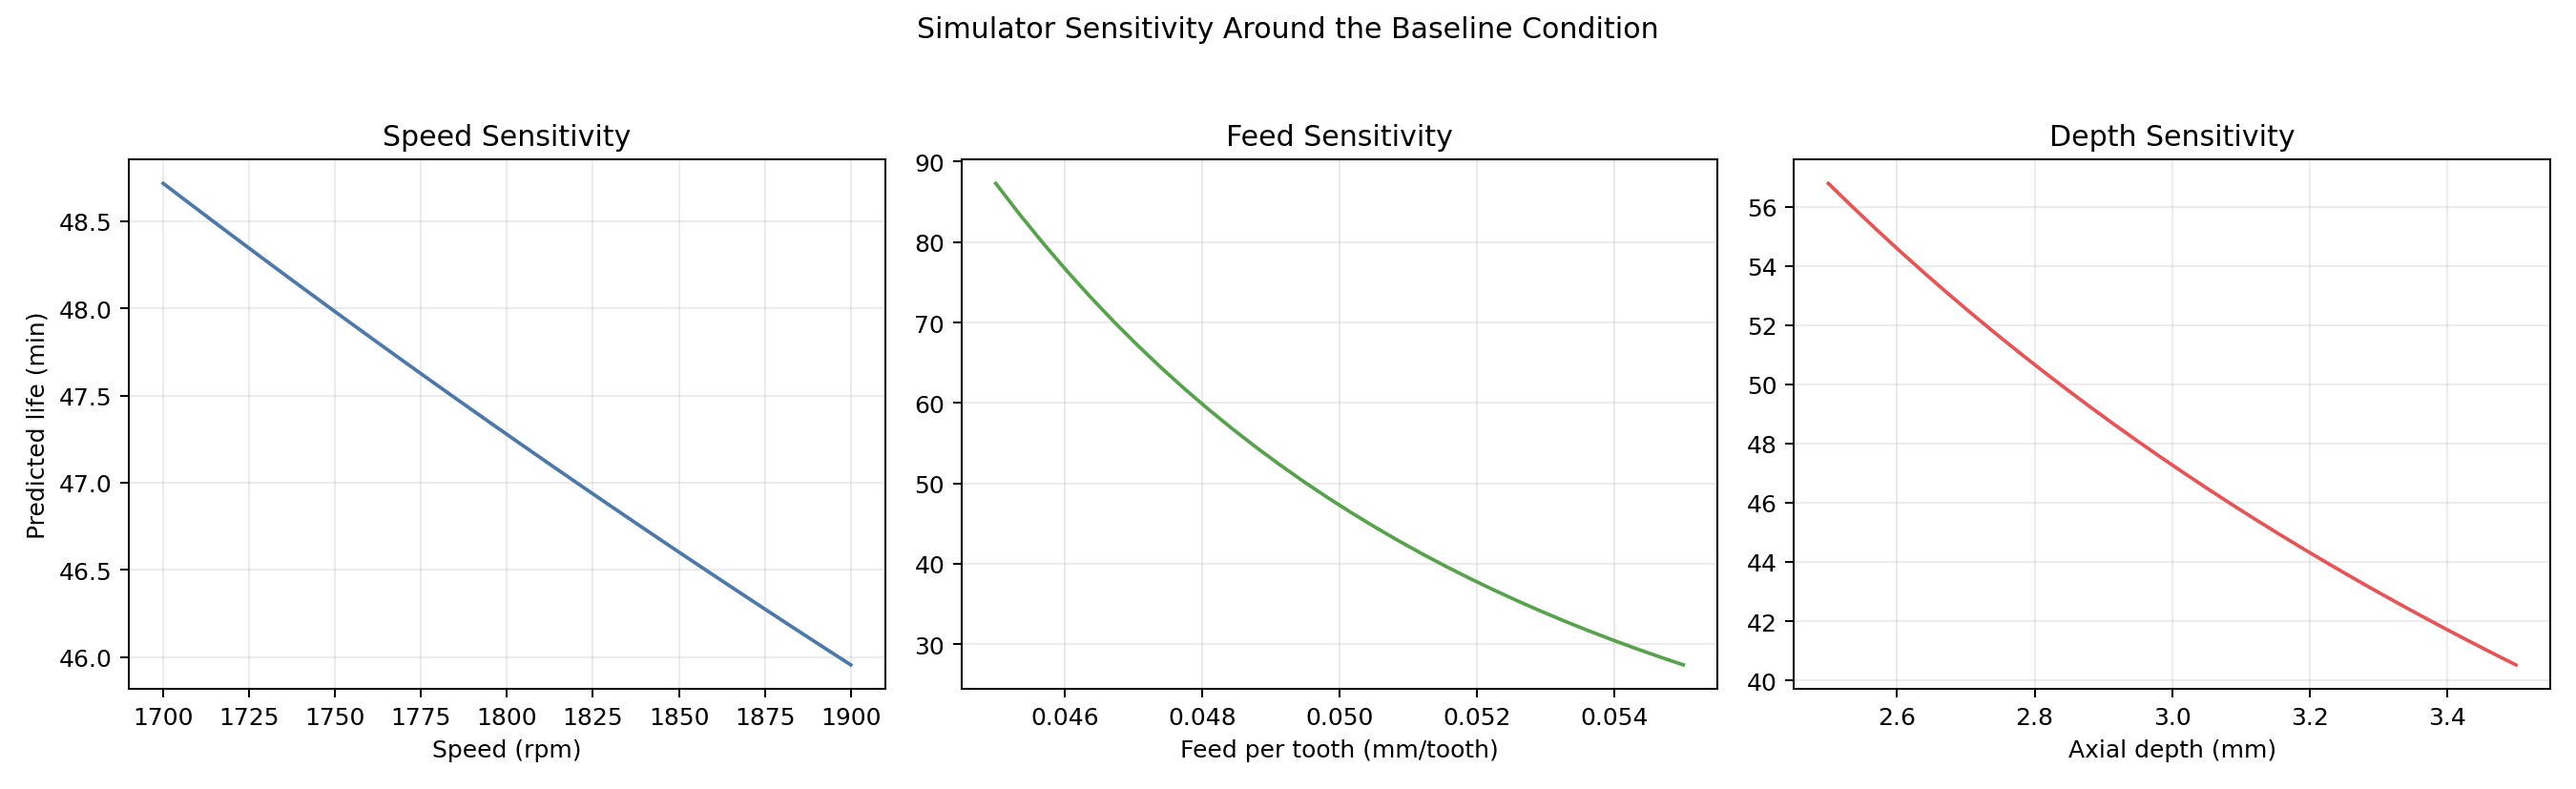
\includegraphics[width=\textwidth,height=0.22\textheight,keepaspectratio]{life_sensitivity_curves.png}
    \caption{Life sensitivity curves}
  \end{subfigure}
  \caption{Feed dominates the local life sensitivity, while speed and depth remain less stable because of narrower design variation and collinearity.}
  \label{fig:condition-law}
\end{figure*}

\subsection{Material effects}

NASA is treated as a separate late-stage and material source. Its feed units, material families, fixed speed and wear scale differ from NUAA, so direct pooling would be unsafe. The NASA late-stage comparison suggests that steel has a stronger late-stage wear factor than cast iron in the local model. This material evidence is used to keep the simulator from treating all late-stage wear as material-independent acceleration.

\begin{figure}[!htbp]
  \centering
  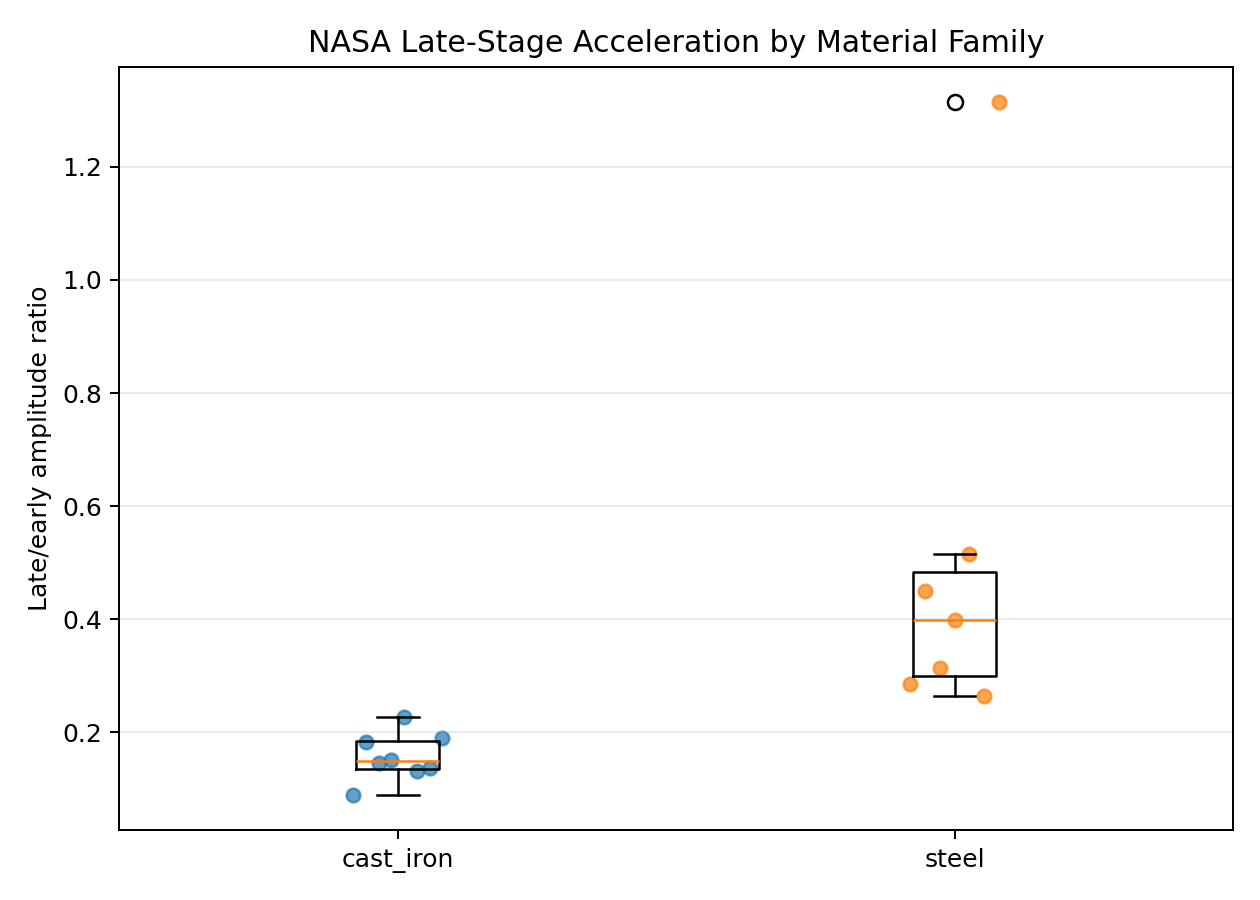
\includegraphics[width=\columnwidth]{nasa_late_stage_materials.png}
  \caption{NASA late-stage material behavior. Steel shows a stronger late-stage factor in the local model.}
  \label{fig:nasa-materials}
\end{figure}

\section{Model validation and results}

\subsection{NASA sensor-modeling benchmark}

The initial single-dataset modeling pass used the NASA milling records to test whether hand-crafted sensor features could predict flank wear under case-held-out validation. The inventory contained 167 runs, of which 146 included \(\vb\) labels across 16 cases. The observed wear range was \(0.000\)--\(1.530~\mathrm{mm}\), with mean \(0.338~\mathrm{mm}\) and standard deviation \(0.261~\mathrm{mm}\). Before modal decomposition, the strongest simple raw-feature association with wear was \code{vib\_spindle\_kurtosis} with \(r=0.3823\). This early result motivated the later use of frequency and modal descriptors rather than relying only on raw amplitude summaries.

\begin{table}[!htbp]
  \centering
  \caption{NASA leave-one-case-out wear-regression benchmark using 29 engineered features.}
  \label{tab:nasa-initial-benchmark}
  \scriptsize
  \begin{tabular}{lrrrr}
    \toprule
    Model & RMSE & MAE & \(R^2\) & MAPE \\
    \midrule
    XGBoost & 0.1892 & 0.1500 & -0.0451 & 48.4\% \\
    SVR & 0.2114 & 0.1733 & -0.1602 & 61.1\% \\
    Random Forest & 0.1758 & 0.1429 & 0.1824 & 47.8\% \\
    Gradient Boosting & 0.1847 & 0.1460 & 0.0287 & 50.1\% \\
    \bottomrule
  \end{tabular}
\end{table}

The best initial NASA regressor was Random Forest, but the modest \(R^2\) and high percentage error showed that a direct black-box wear regressor was not sufficient for replacement planning. That finding is carried forward into the rest of the work: all later model comparisons use grouped validation, dataset-specific thresholds and explicit checks for whether low wear error transfers into useful life estimates.

\subsection{Cross-dataset health baselines}

The cross-dataset pipeline evaluates wear regression and failure classification with grouped validation. Grouped validation is essential because adjacent samples from the same cutter or case are not independent deployment tests. The goal is to estimate transfer to unseen experiments rather than interpolation inside one trajectory.

\begin{table}[!htbp]
  \centering
  \caption{Cross-dataset wear regression and failure classification.}
  \label{tab:cross-dataset-metrics}
  \scriptsize
  \begin{tabular}{lrrrr}
    \toprule
    Dataset & Samples & Features & RMSE & ROC-AUC \\
    \midrule
    PHM2010 & 945 & 105 & 0.0181 & 0.9671 \\
    NASA & 146 & 94 & 0.1728 & 0.9141 \\
    UniWear & 649 & 46 & 0.0475 & 0.7350 \\
    \bottomrule
  \end{tabular}
\end{table}

\begin{figure*}[!t]
  \centering
  \begin{subfigure}[t]{0.49\textwidth}
    \centering
    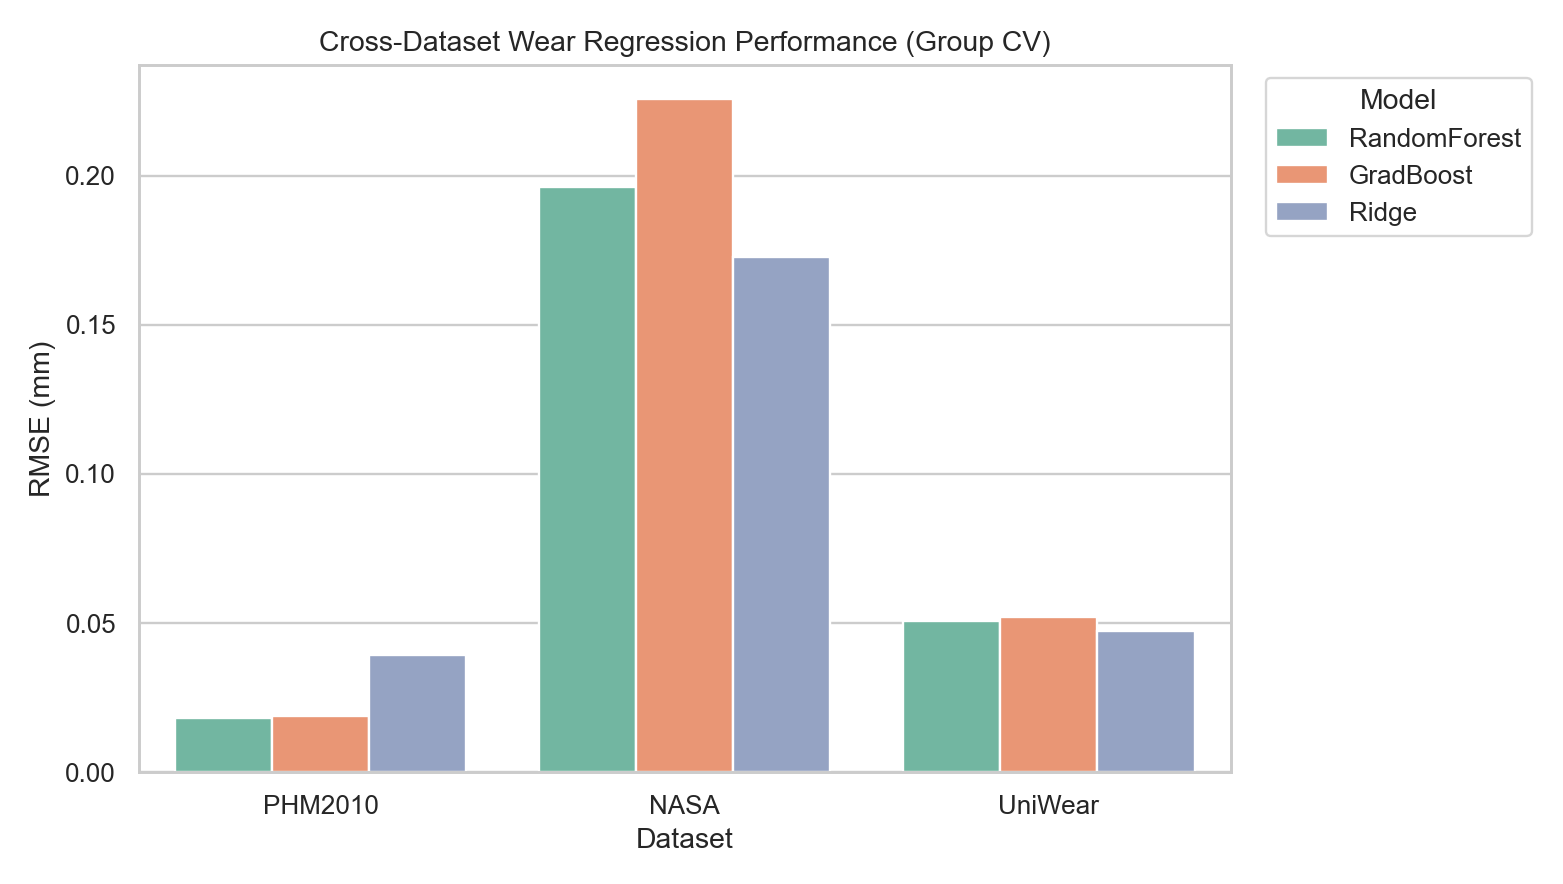
\includegraphics[width=\textwidth]{cross_dataset_rmse_comparison.png}
    \caption{Regression RMSE}
  \end{subfigure}
  \hfill
  \begin{subfigure}[t]{0.49\textwidth}
    \centering
    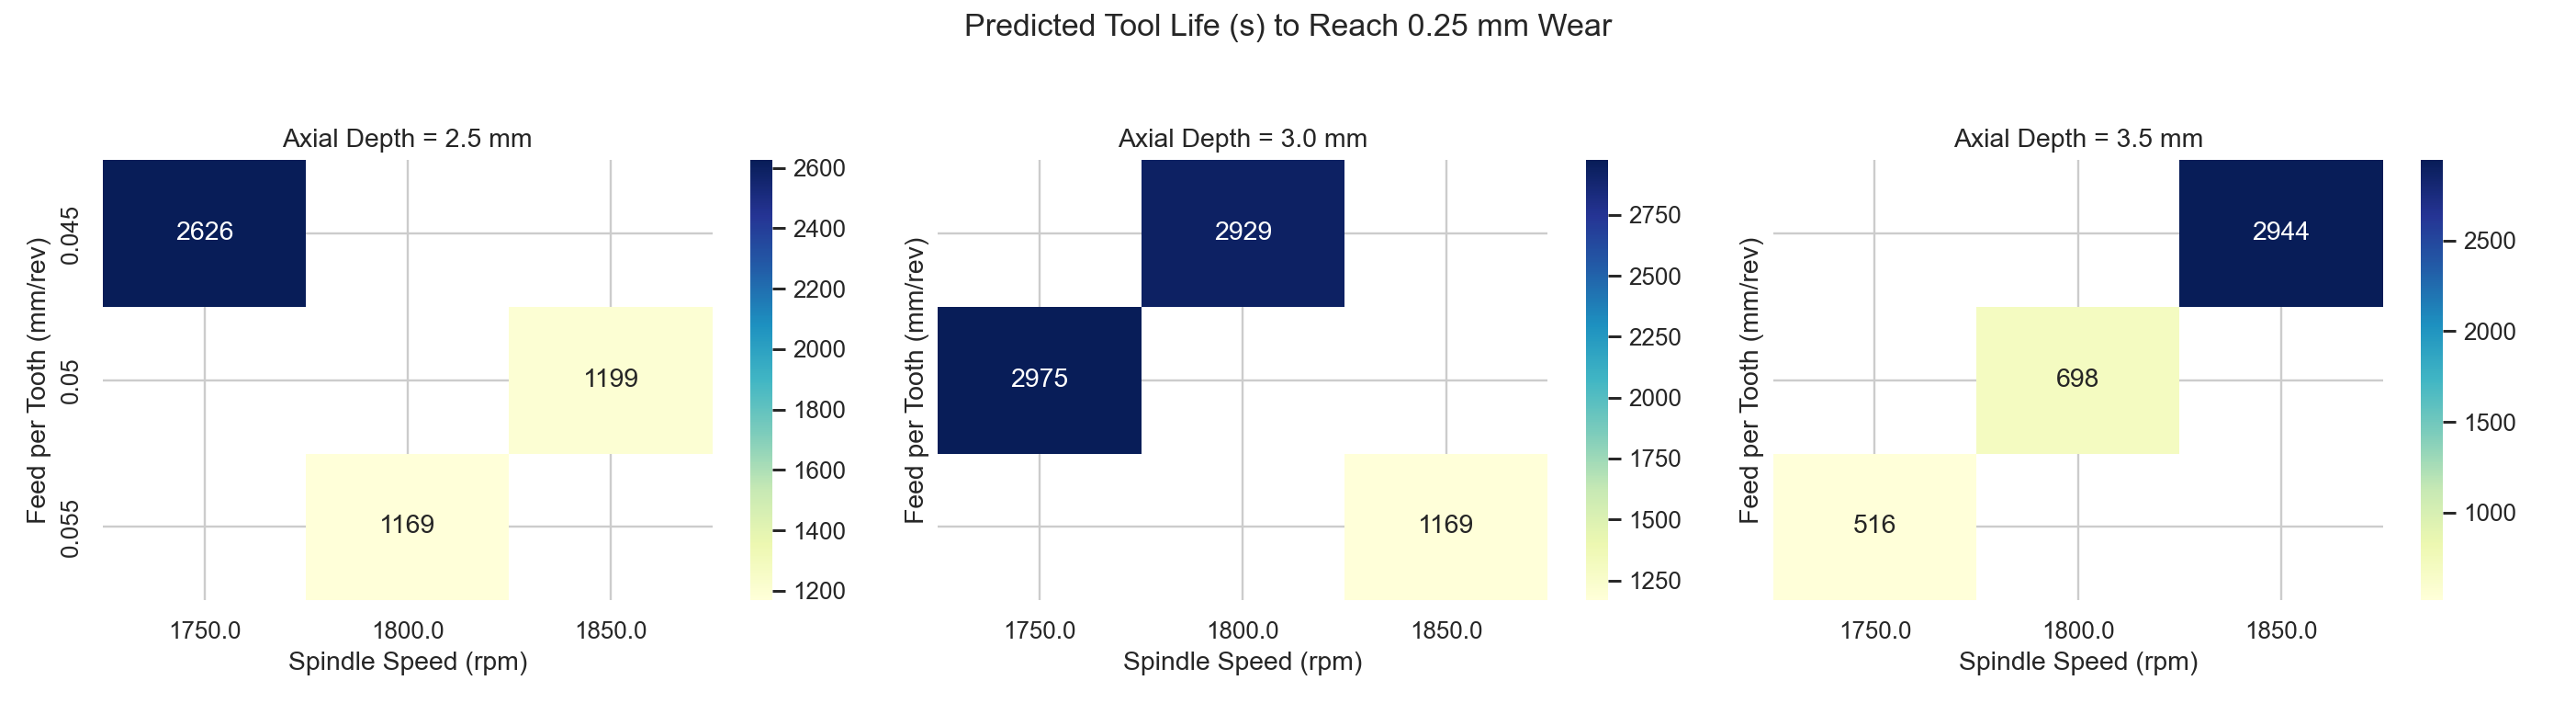
\includegraphics[width=\textwidth]{nuaa_life_heatmap.png}
    \caption{NUAA life heatmap}
  \end{subfigure}
  \caption{Cross-dataset baselines and process-condition sensitivity. NASA remains the hardest local regression regime because it includes material variation and severe wear.}
  \label{fig:cross-dataset-baselines}
\end{figure*}

The failure-marker plots show that failure labels are usually preceded by increasing energy, dispersion or impulsiveness, but the exact marker family varies by dataset. This is consistent with machining physics: tool wear changes chip formation, friction, heat generation and dynamic stiffness, and the resulting evidence can appear in vibration, acoustic emission, force/current or frequency features depending on the available sensors.

\begin{figure*}[!t]
  \centering
  \begin{subfigure}[t]{0.32\textwidth}
    \centering
    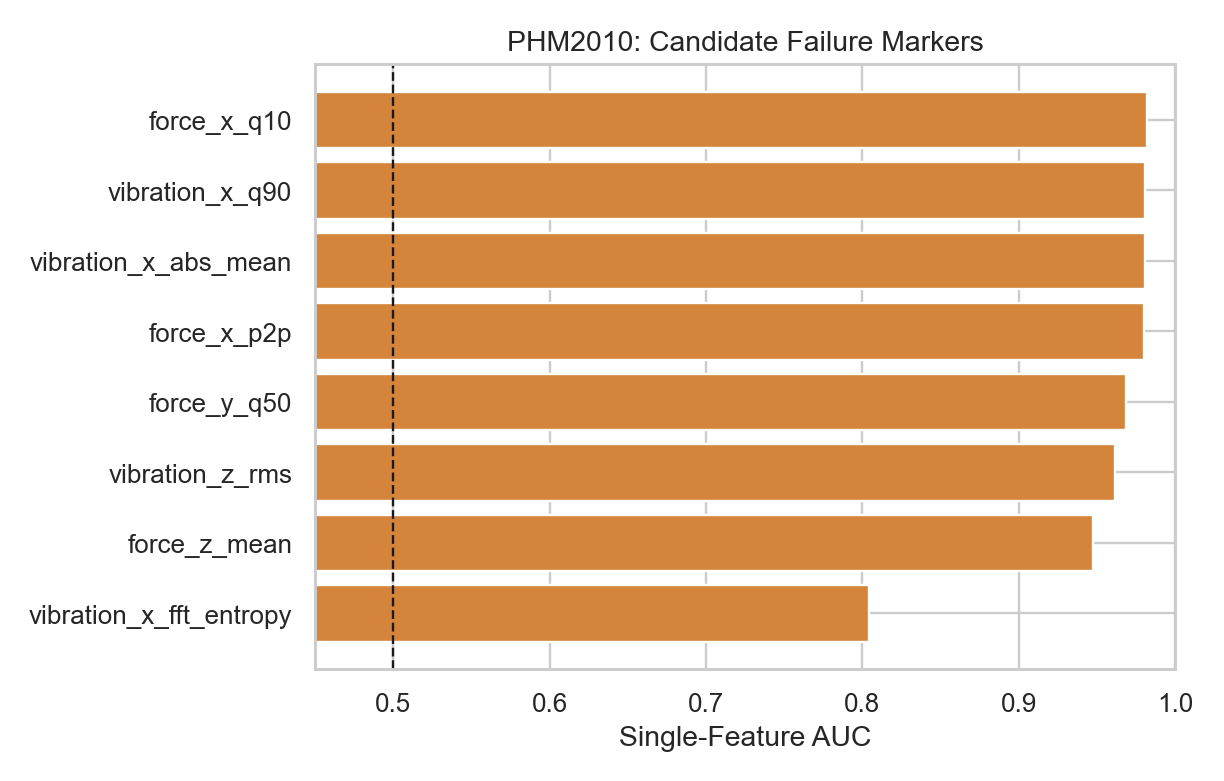
\includegraphics[width=\textwidth]{phm2010_failure_markers.png}
    \caption{PHM2010}
  \end{subfigure}
  \hfill
  \begin{subfigure}[t]{0.32\textwidth}
    \centering
    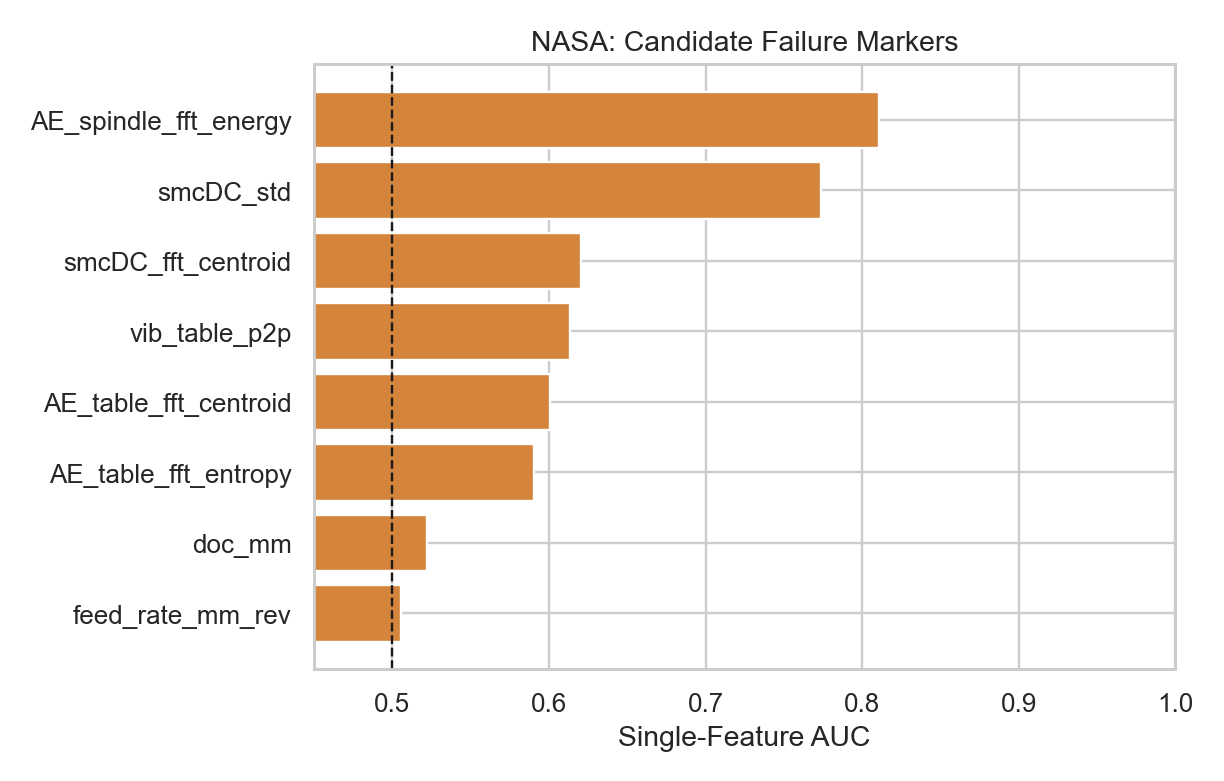
\includegraphics[width=\textwidth]{nasa_failure_markers.png}
    \caption{NASA}
  \end{subfigure}
  \hfill
  \begin{subfigure}[t]{0.32\textwidth}
    \centering
    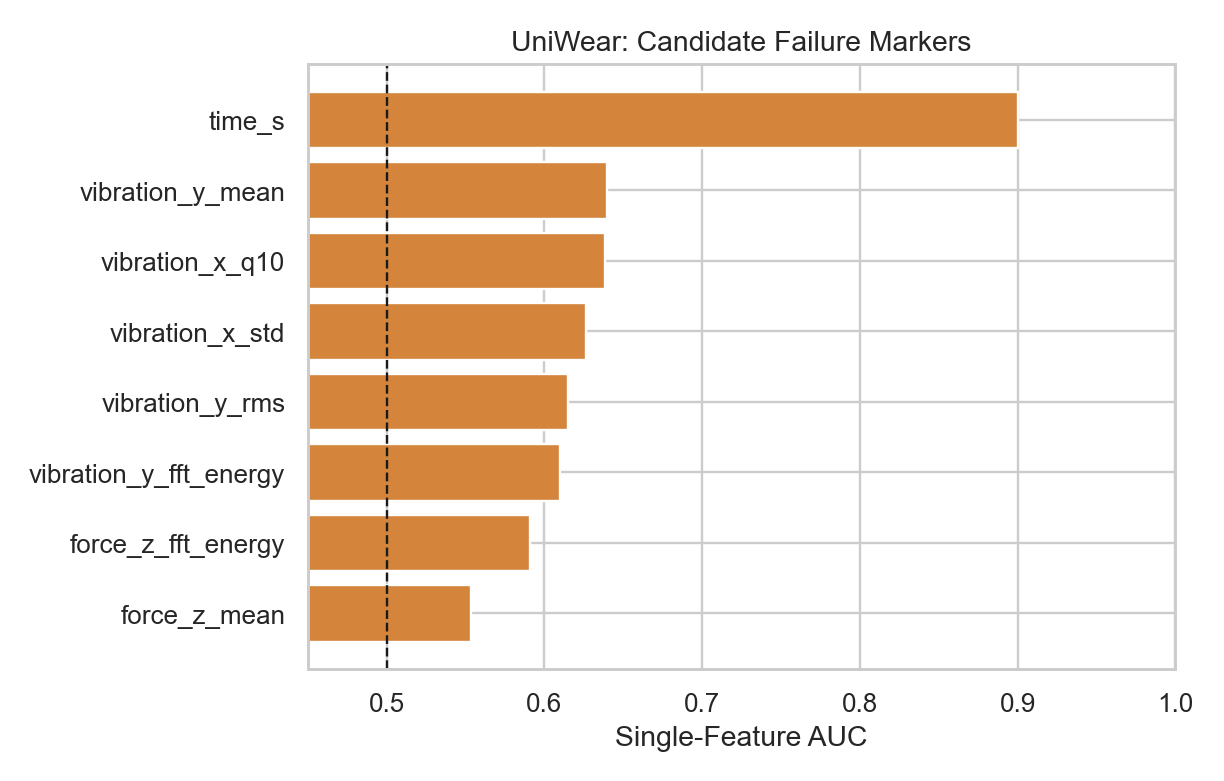
\includegraphics[width=\textwidth]{uniwear_failure_markers.png}
    \caption{UniWear}
  \end{subfigure}
  \caption{Failure-marker summaries across datasets. The plots support energy, dispersion, crest and modal frequency indicators as health signals.}
  \label{fig:failure-markers}
\end{figure*}

\subsection{Coefficient uncertainty}

The extended research pass bootstraps the NUAA condition law with valid-design filtering. This is necessary because small experimental designs can produce rank-deficient or unstable resamples. The results show a stable feed exponent, while speed and depth remain more uncertain.

\begin{table}[!htbp]
  \centering
  \caption{Bootstrap coefficient summary for the NUAA condition law.}
  \label{tab:bootstrap-coefficients}
  \scriptsize
  \begin{tabular}{lrrr}
    \toprule
    Quantity & 2.5\% & Median & 97.5\% \\
    \midrule
    \(k_{\mathrm{early}}\) & 0.01558 & 0.01783 & 0.02183 \\
    Speed exponent & -7.49808 & 1.16739 & 8.04424 \\
    Feed exponent & 2.04563 & 3.99243 & 6.68021 \\
    Depth exponent & -0.59012 & 0.51957 & 1.92473 \\
    Amplitude \(R^2\) & -- & 0.89715 & -- \\
    \bottomrule
  \end{tabular}
\end{table}

\begin{figure}[!htbp]
  \centering
  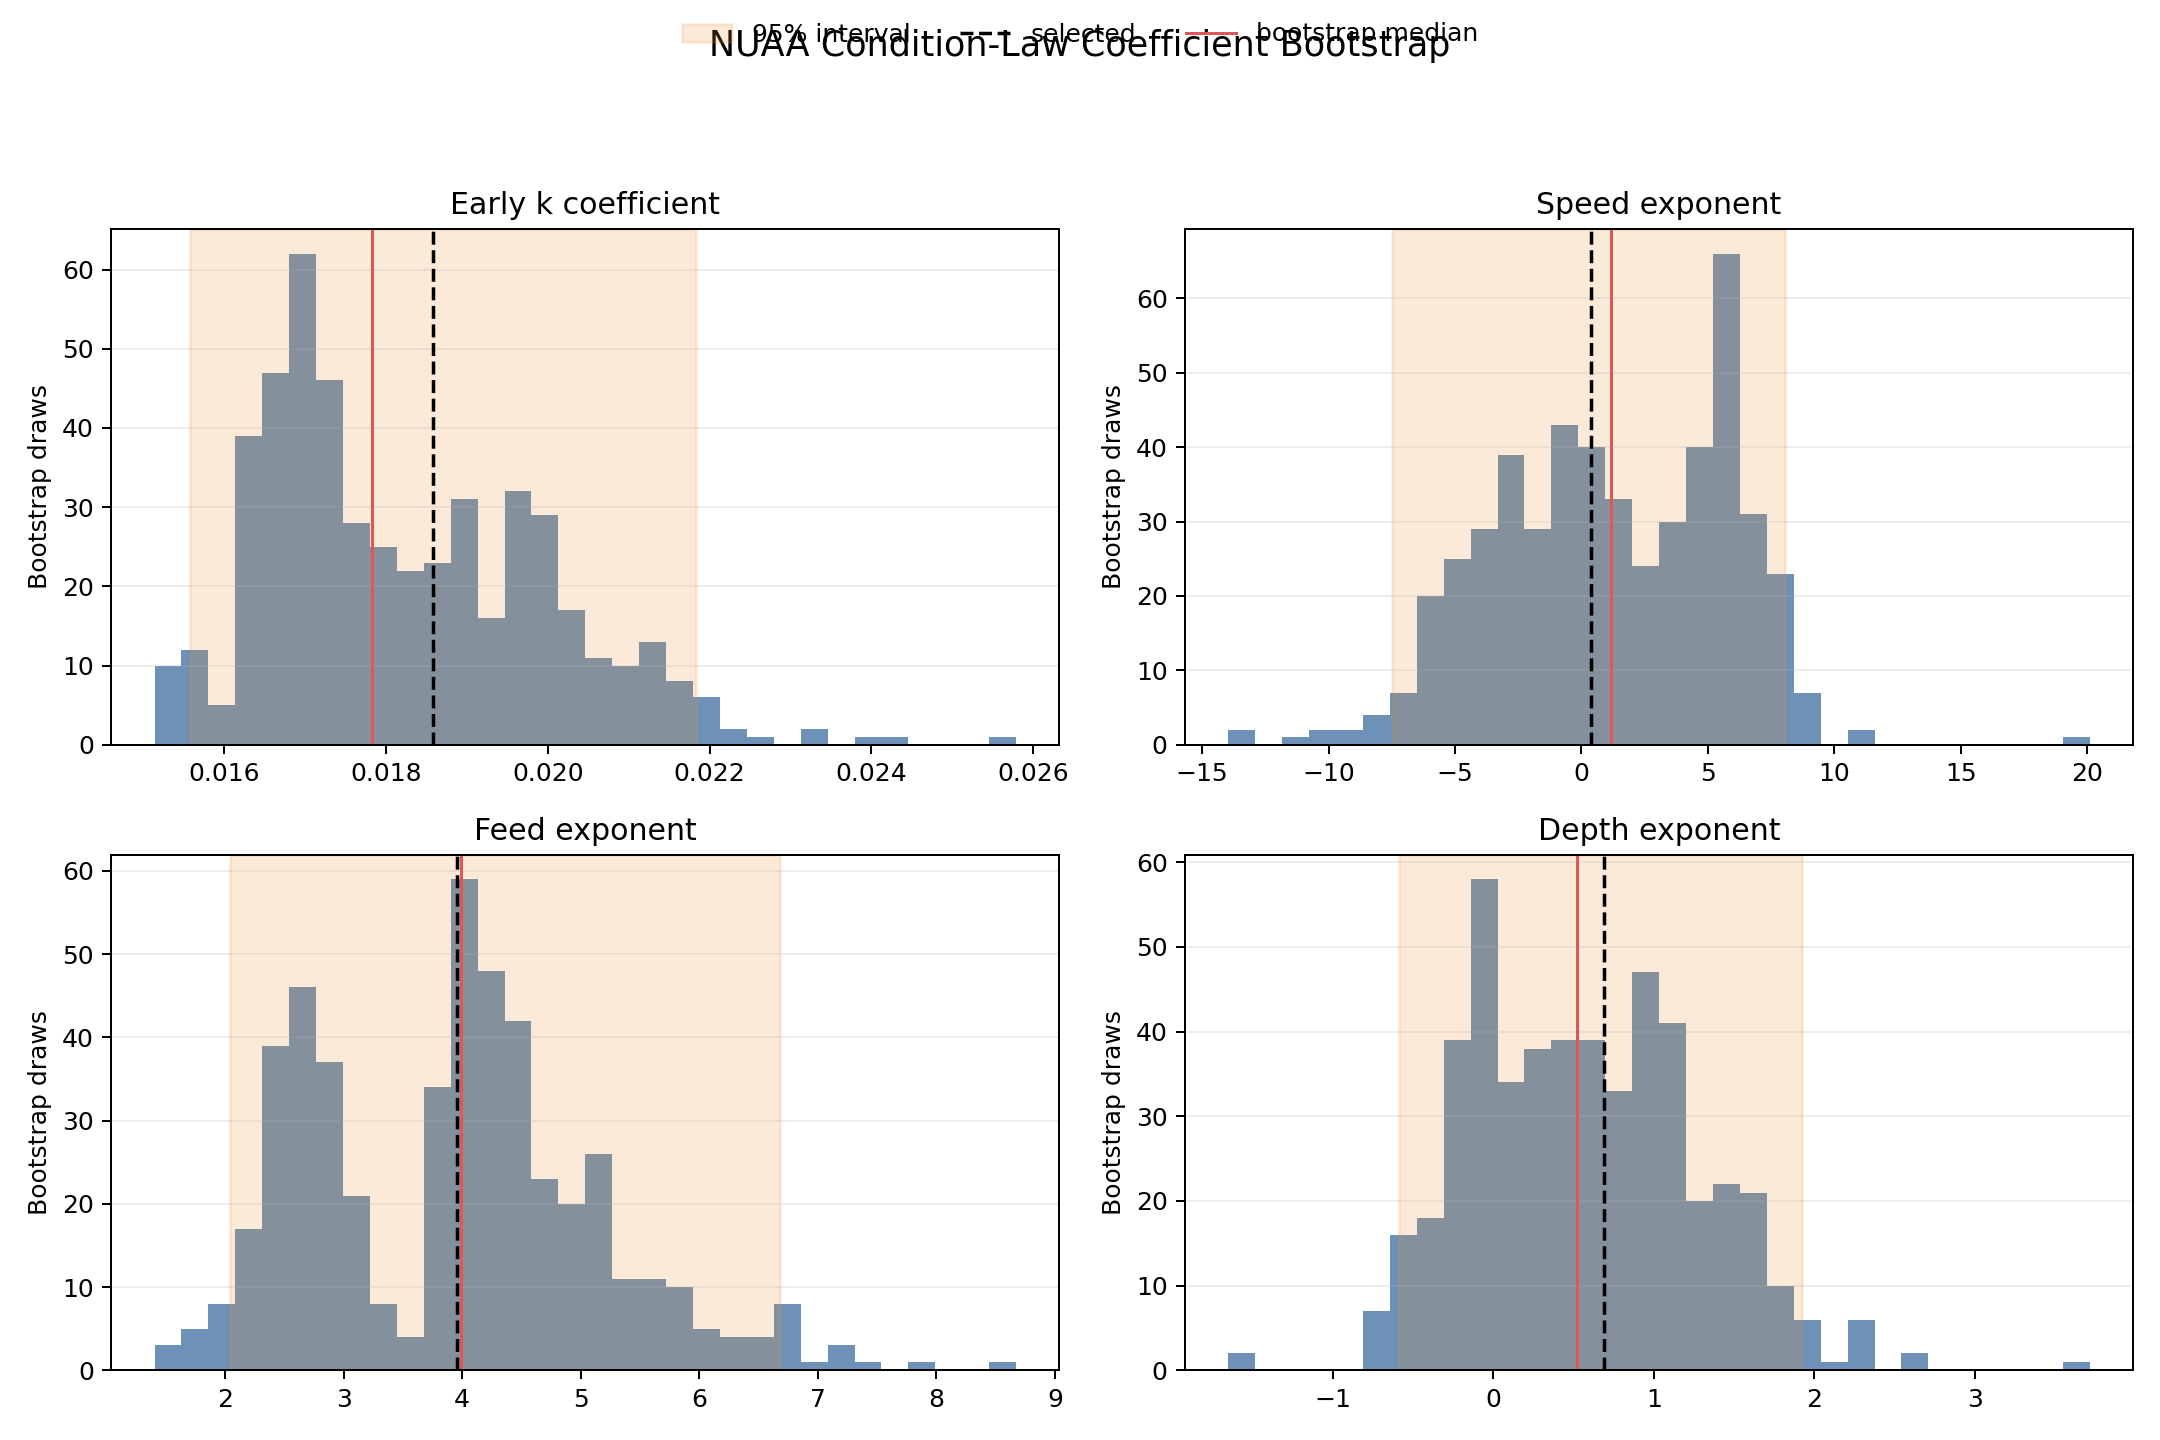
\includegraphics[width=\columnwidth]{condition_coefficient_bootstrap.png}
  \caption{Bootstrap distributions for condition-law coefficients. Feed is the most consistently identified operating variable.}
  \label{fig:bootstrap-coefficients}
\end{figure}

\subsection{Life intervals and calibration}

Bootstrap draws are propagated into low-load, baseline and high-load life scenarios. The baseline median life is about 50.2 min. The low-load condition extends median life to about 103.6 min, while the high-load condition compresses median life to about 25.0 min.

\begin{table}[!htbp]
  \centering
  \caption{Bootstrap life prediction intervals.}
  \label{tab:life-intervals}
  \scriptsize
  \begin{tabular}{lrrrrrr}
    \toprule
    Scenario & Speed & Feed & Depth & 2.5\% & Median & 97.5\% \\
    \midrule
    Low load & 1750 & 0.045 & 2.5 & 59.797 & 103.644 & 247.675 \\
    Baseline & 1800 & 0.050 & 3.0 & 37.422 & 50.227 & 61.177 \\
    High load & 1850 & 0.055 & 3.5 & 11.514 & 24.987 & 38.046 \\
    \bottomrule
  \end{tabular}
\end{table}

\begin{figure}[!htbp]
  \centering
  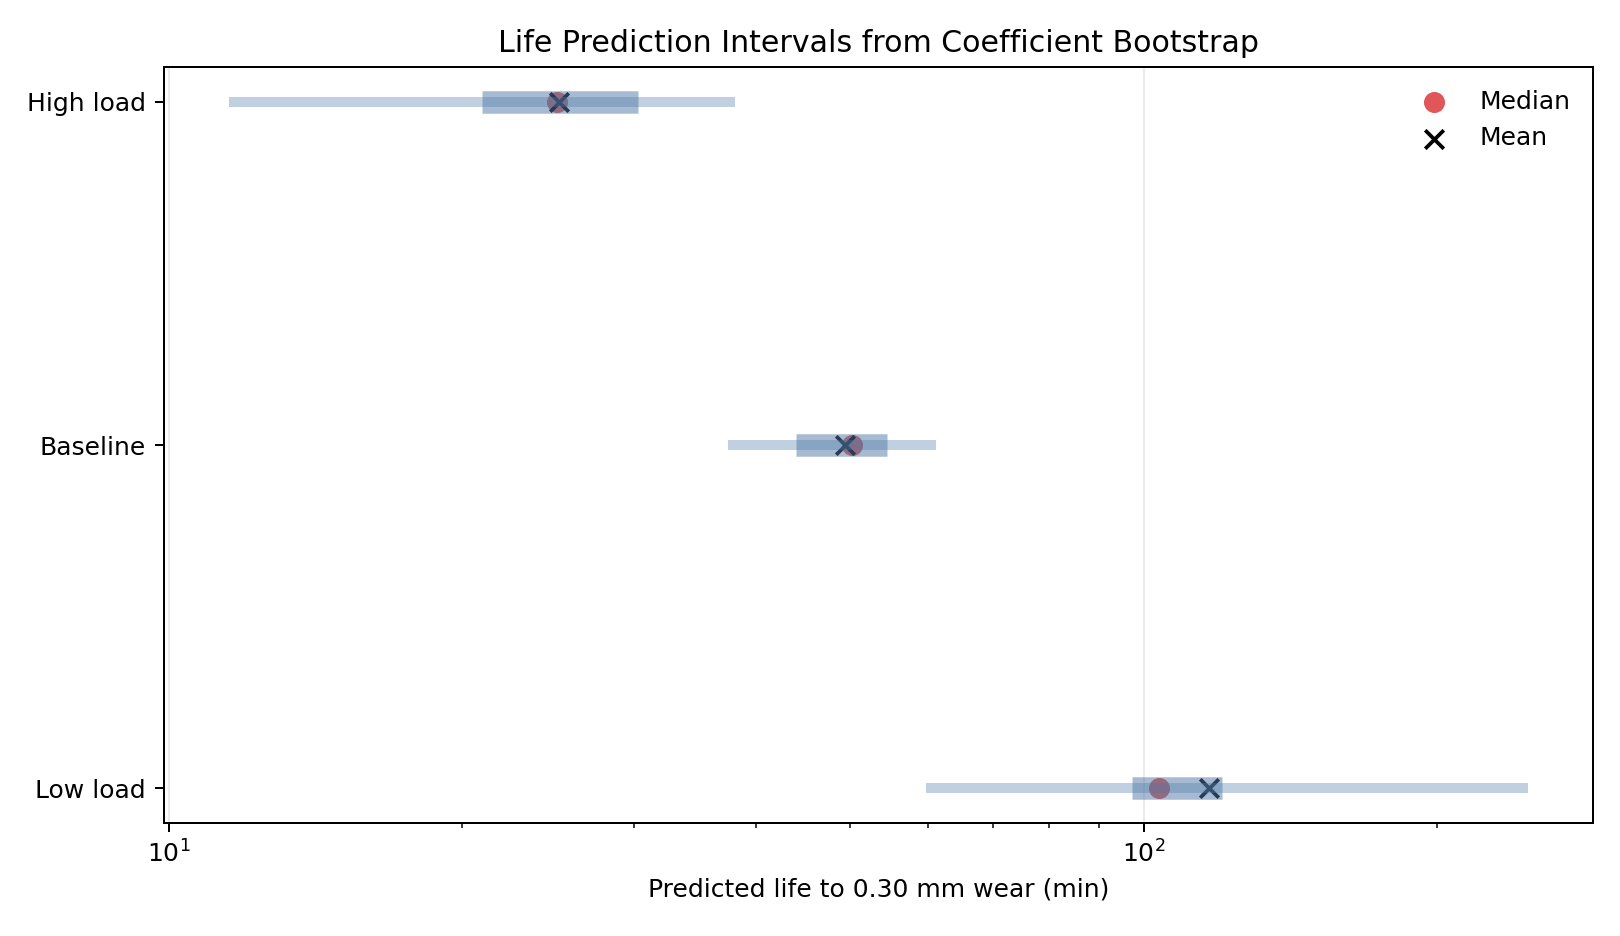
\includegraphics[width=\columnwidth]{life_prediction_intervals.png}
  \caption{Load-dependent life intervals. The high-load scenario roughly halves baseline median life.}
  \label{fig:life-intervals}
\end{figure}

The project also tested whether early observations from each run could calibrate the global equation through a per-run multiplier. The result was negative for the local NUAA holdout. At cutoff fractions of 0.25, 0.40 and 0.60, calibrated RMSE values were 0.05045, 0.04750 and 0.04230, while uncalibrated RMSE values were 0.04047, 0.02508 and 0.02819. This prevents an overly optimistic simulator story: short-window scalar calibration can overcorrect the global model. Future calibration should use monotonic constraints, Bayesian updating or a state-space formulation.

\begin{figure}[!htbp]
  \centering
  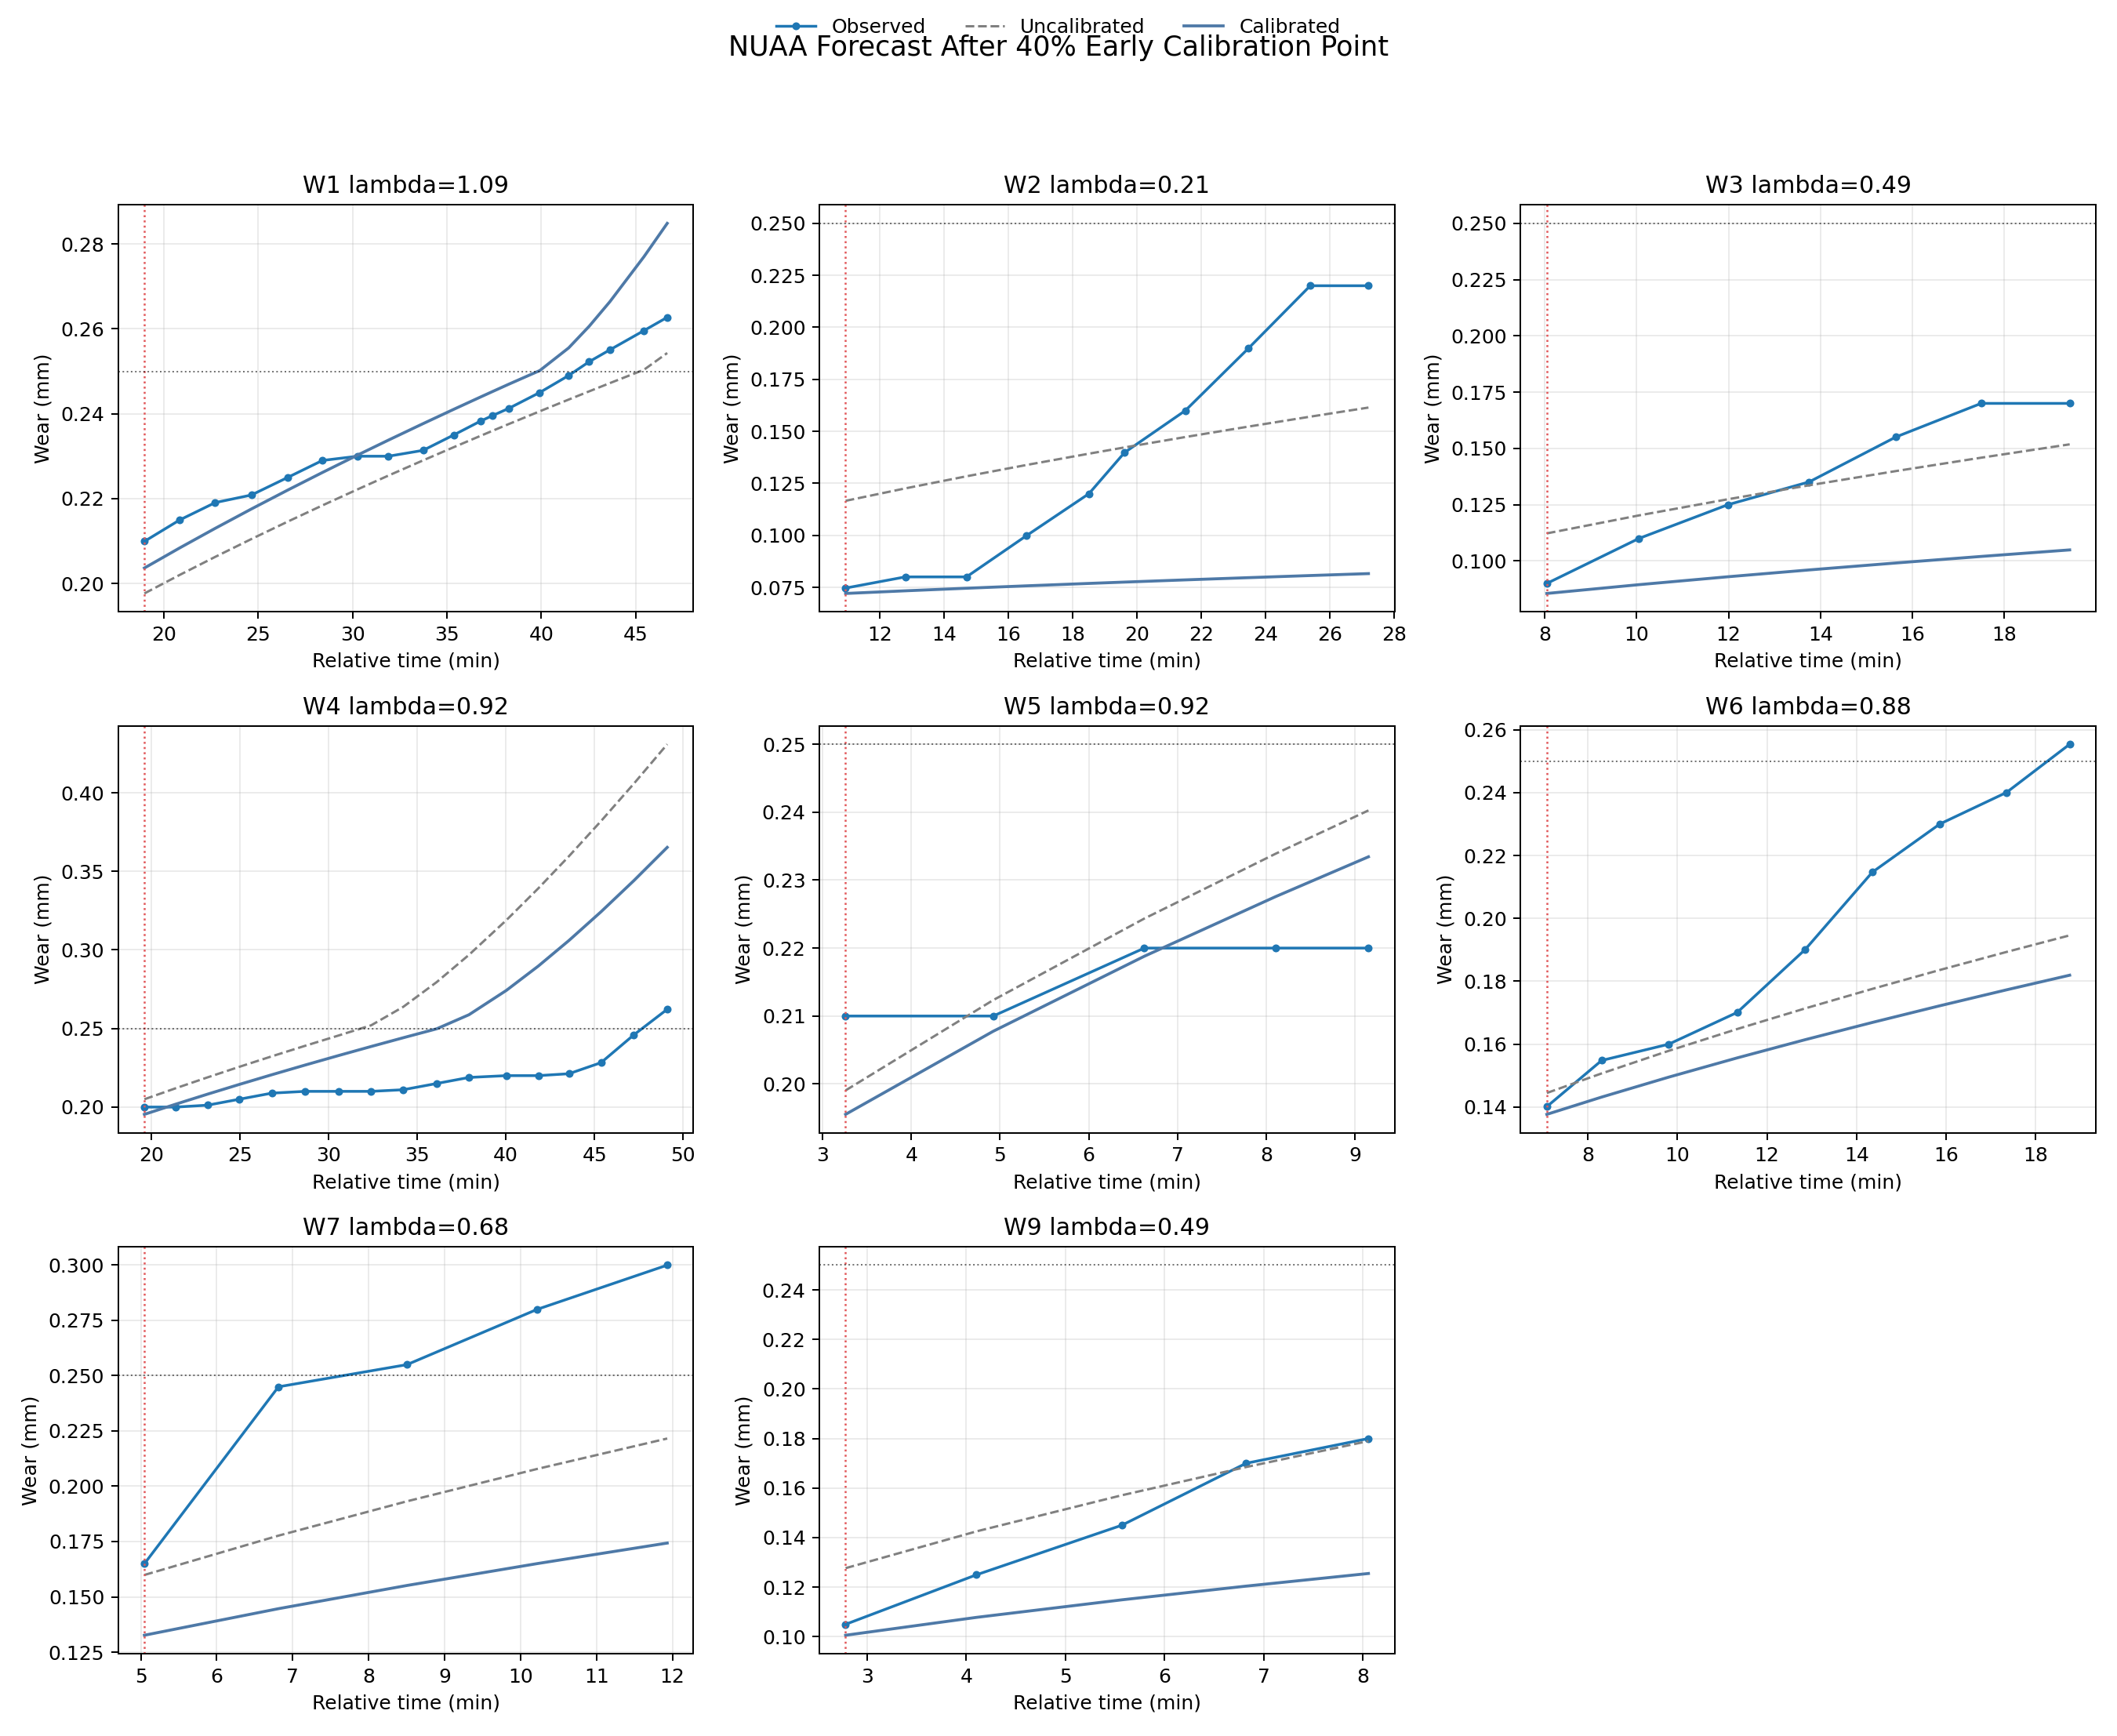
\includegraphics[width=\columnwidth]{nuaa_calibration_forecast.png}
  \caption{NUAA calibration diagnostic. Short-window scalar calibration can worsen holdout forecasts.}
  \label{fig:nuaa-calibration}
\end{figure}

\subsection{Residual diagnostics}

Residual diagnostics show that the piecewise equation is most accurate in PHM2010 and NUAA early regimes, and least accurate in NASA, where severe wear, material variation and late-stage behavior are stronger.

\begin{table}[!htbp]
  \centering
  \caption{Residual diagnostics for the piecewise wear equation.}
  \label{tab:residual-diagnostics}
  \scriptsize
  \begin{tabular}{lrrrrr}
    \toprule
    Dataset & Points & Bias & MAE & RMSE & 95\% abs. \\
    \midrule
    NASA & 146 & 0.00763 & 0.03149 & 0.04376 & 0.08825 \\
    NUAA & 152 & -0.00162 & 0.01568 & 0.02113 & 0.04087 \\
    PHM2010 & 945 & 0.00104 & 0.01070 & 0.01362 & 0.02437 \\
    \bottomrule
  \end{tabular}
\end{table}

\begin{figure}[!htbp]
  \centering
  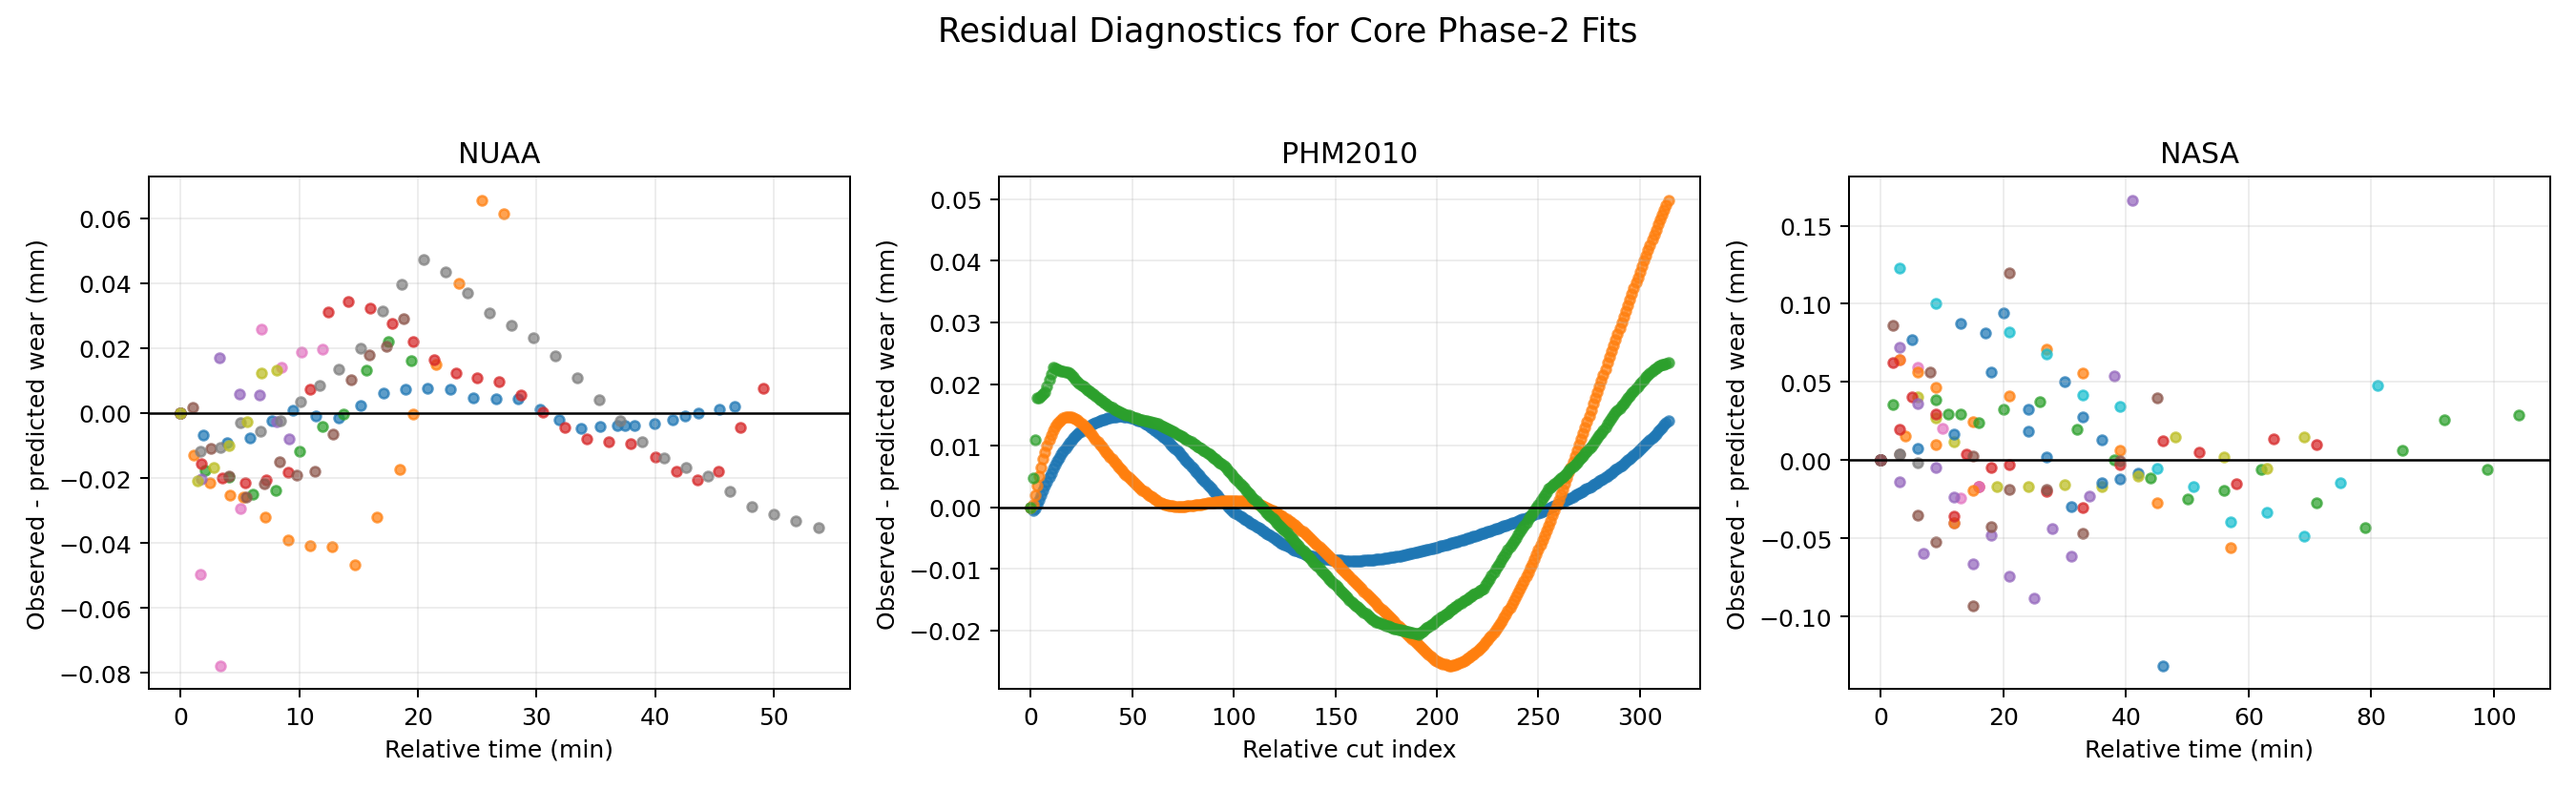
\includegraphics[width=\columnwidth]{residual_diagnostics.png}
  \caption{Residual diagnostics across datasets. The NASA tail remains the hardest local regime.}
  \label{fig:residual-diagnostics}
\end{figure}

\section{Lifetime modeling}

\subsection{Threshold labels}

The lifetime rework directly addresses whether tool life can be estimated by training models and extracting results from those models. It can, but the target changes. Life labels are built by finding when each run crosses a dataset-specific wear threshold. Runs that do not cross before the observation end are treated as censored. NUAA and NASA lives are in minutes, while PHM2010 uses cutter cut index because its native time base differs.

\begin{table}[!htbp]
  \centering
  \caption{Threshold-crossing life labels.}
  \label{tab:life-labels}
  \scriptsize
  \begin{tabular}{lrrrr}
    \toprule
    Dataset & Records & Threshold & Events & Censored \\
    \midrule
    NUAA & 9 & 0.250 mm & 5 & 4 \\
    NASA & 15 & 0.300 mm & 15 & 0 \\
    PHM2010 & 3 & 0.150 mm & 3 & 0 \\
    \bottomrule
  \end{tabular}
\end{table}

\subsection{Training wear models and inverting life}

NUAA wear models are trained under leave-one-experiment-out validation and then inverted to estimate threshold-crossing life. The inversion step exposes a negative result that is important for model selection. Gradient Boosting has the best pointwise wear RMSE, but its event-life MAE is worse than the compact piecewise equation and Ridge. Therefore, the lifetime problem cannot be judged only by \(\vb\) regression error. Smoothness and bias near the threshold matter.

\begin{table*}[!t]
  \centering
  \caption{NUAA trained wear models and inverted event-life performance.}
  \label{tab:wear-life-benchmark}
  \footnotesize
  \begin{tabular}{lrrrrr}
    \toprule
    Model & Wear RMSE & Wear MAE & Wear \(R^2\) & Event-life MAE & Censor-bound rate \\
    \midrule
    PiecewiseEquation & 0.0969 & 0.0460 & -0.8811 & 5.3832 & 1.00 \\
    Ridge & 0.0505 & 0.0407 & 0.4883 & 6.7010 & 0.75 \\
    Random Forest & 0.0457 & 0.0337 & 0.5817 & 8.9847 & 1.00 \\
    Gradient Boosting & 0.0394 & 0.0310 & 0.6896 & 11.6555 & 1.00 \\
    Gaussian Process & 0.0607 & 0.0459 & 0.2631 & 16.1923 & 1.00 \\
    MLP & 0.1159 & 0.0956 & -1.6890 & 19.0334 & 0.50 \\
    \bottomrule
  \end{tabular}
\end{table*}

\begin{figure*}[!t]
  \centering
  \begin{subfigure}[t]{0.49\textwidth}
    \centering
    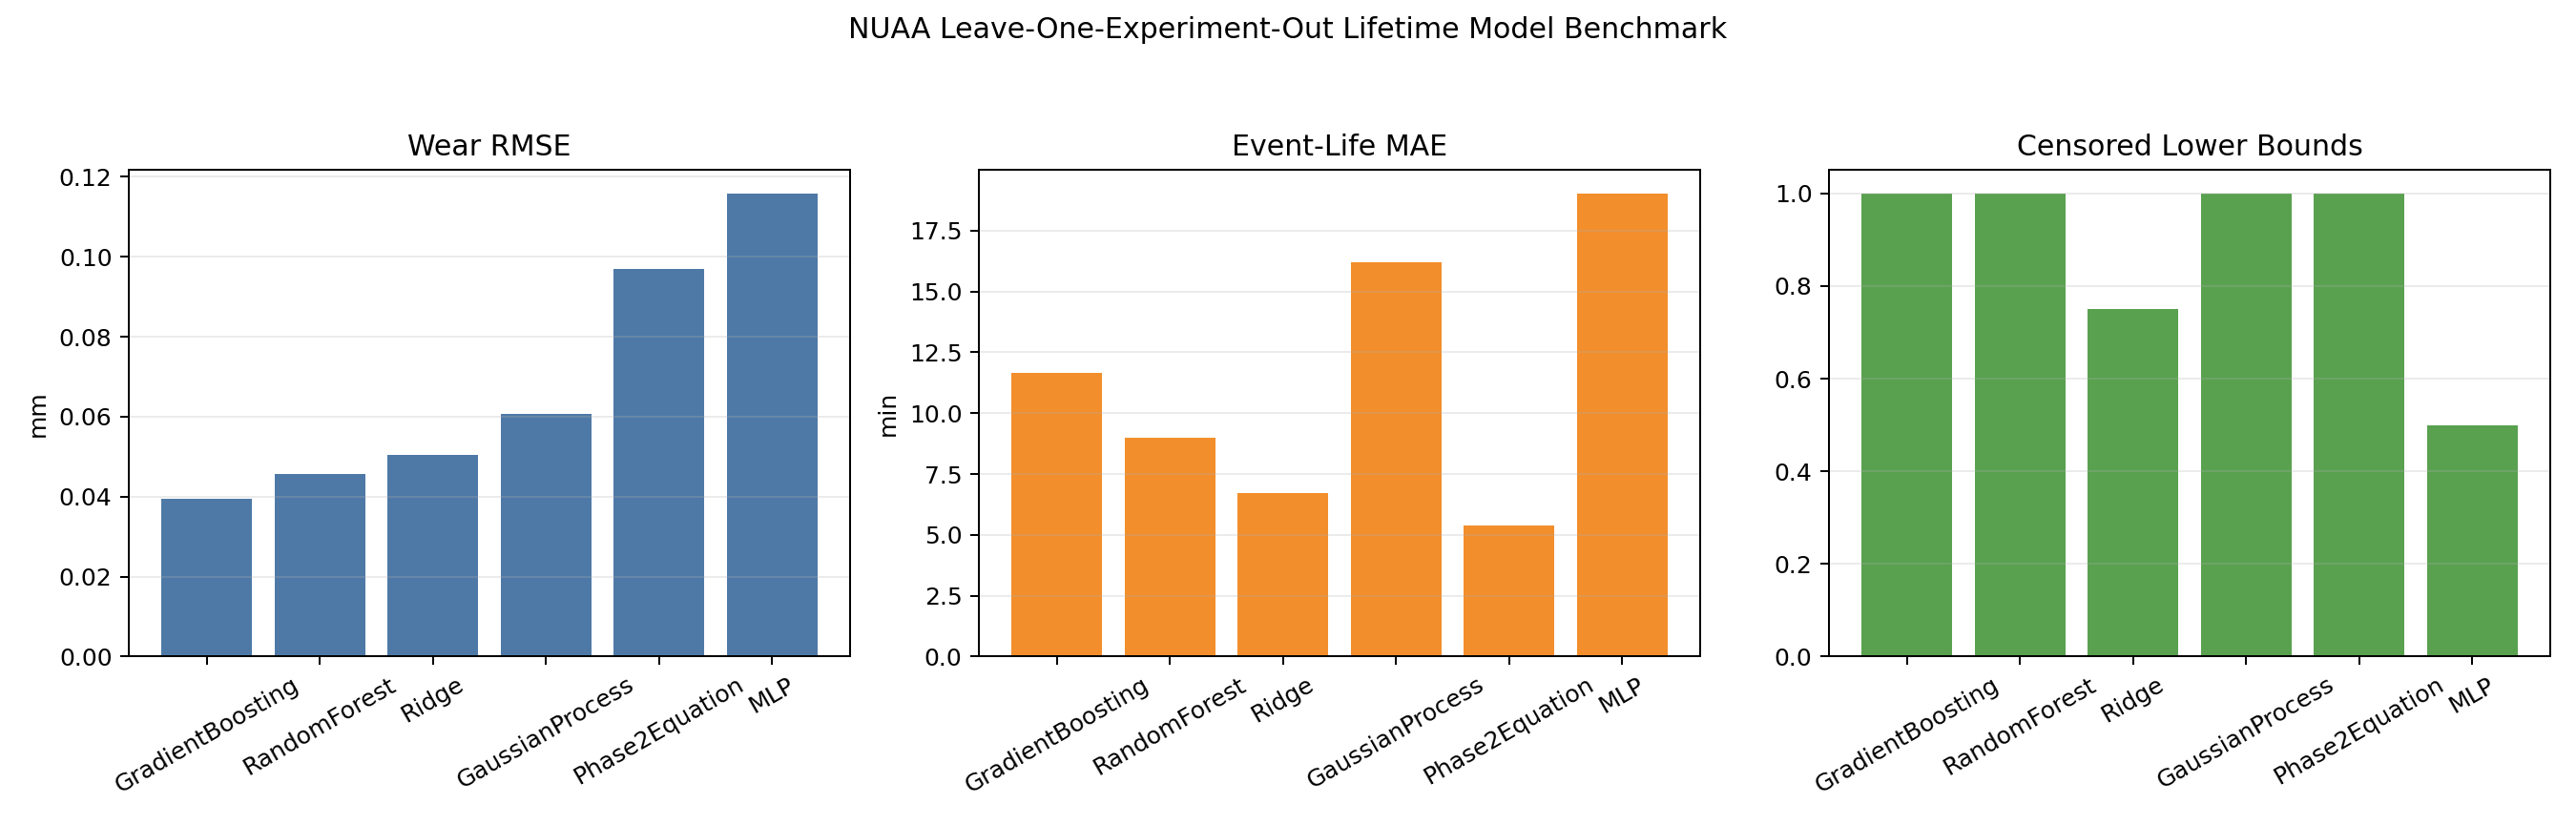
\includegraphics[width=\textwidth]{nuaa_wear_life_model_benchmark.png}
    \caption{Wear and life benchmark}
  \end{subfigure}
  \hfill
  \begin{subfigure}[t]{0.49\textwidth}
    \centering
    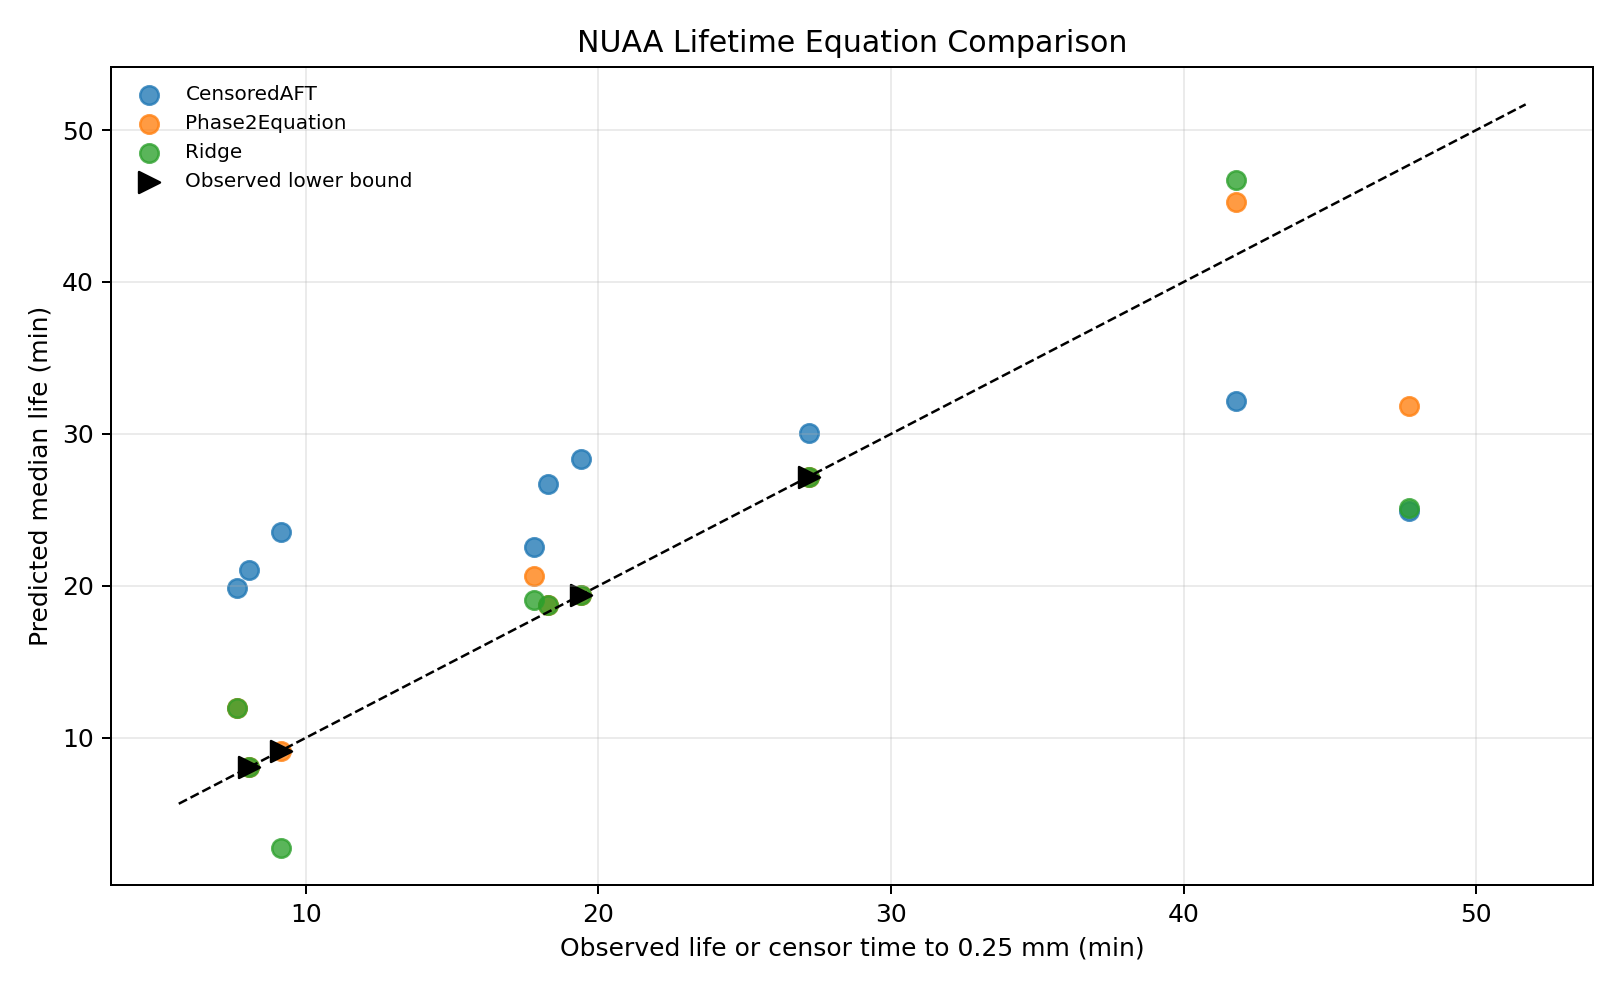
\includegraphics[width=\textwidth]{nuaa_life_equation_comparison.png}
    \caption{Life equation comparison}
  \end{subfigure}
  \caption{Wear-model inversion changes the model-selection problem. Smooth threshold behavior matters.}
  \label{fig:wear-life-benchmark}
\end{figure*}

\subsection{NUAA accelerated-failure-time equation}

The NUAA censored accelerated-failure-time model is
\begin{equation}
T_{\min} =
24.93
\left(\frac{n}{1800}\right)^{-0.0187}
\left(\frac{f_z}{0.05}\right)^{-1.7662}
\left(\frac{a_p}{3.0}\right)^{-0.3768},
\label{eq:nuaa-aft}
\end{equation}
with \(\sigma=0.5291\) and negative log likelihood \(21.2365\). The AFT feed exponent is weaker than the dense condition-law feed exponent because it models sparse threshold-crossing events with censoring, not dense early wear amplitudes.

\begin{table}[!htbp]
  \centering
  \caption{NUAA AFT bootstrap coefficients.}
  \label{tab:aft-bootstrap}
  \scriptsize
  \begin{tabular}{lrrr}
    \toprule
    Coefficient & 2.5\% & Median & 97.5\% \\
    \midrule
    Intercept & 2.7199 & 3.2103 & 3.8286 \\
    log speed & -6.2471 & -0.2186 & 0.9129 \\
    log feed & -7.4945 & -2.1886 & 0.1153 \\
    log depth & -2.4450 & -0.5467 & 4.5558 \\
    sigma & 0.0000 & 0.1826 & 0.6821 \\
    \bottomrule
  \end{tabular}
\end{table}

\begin{figure}[!htbp]
  \centering
  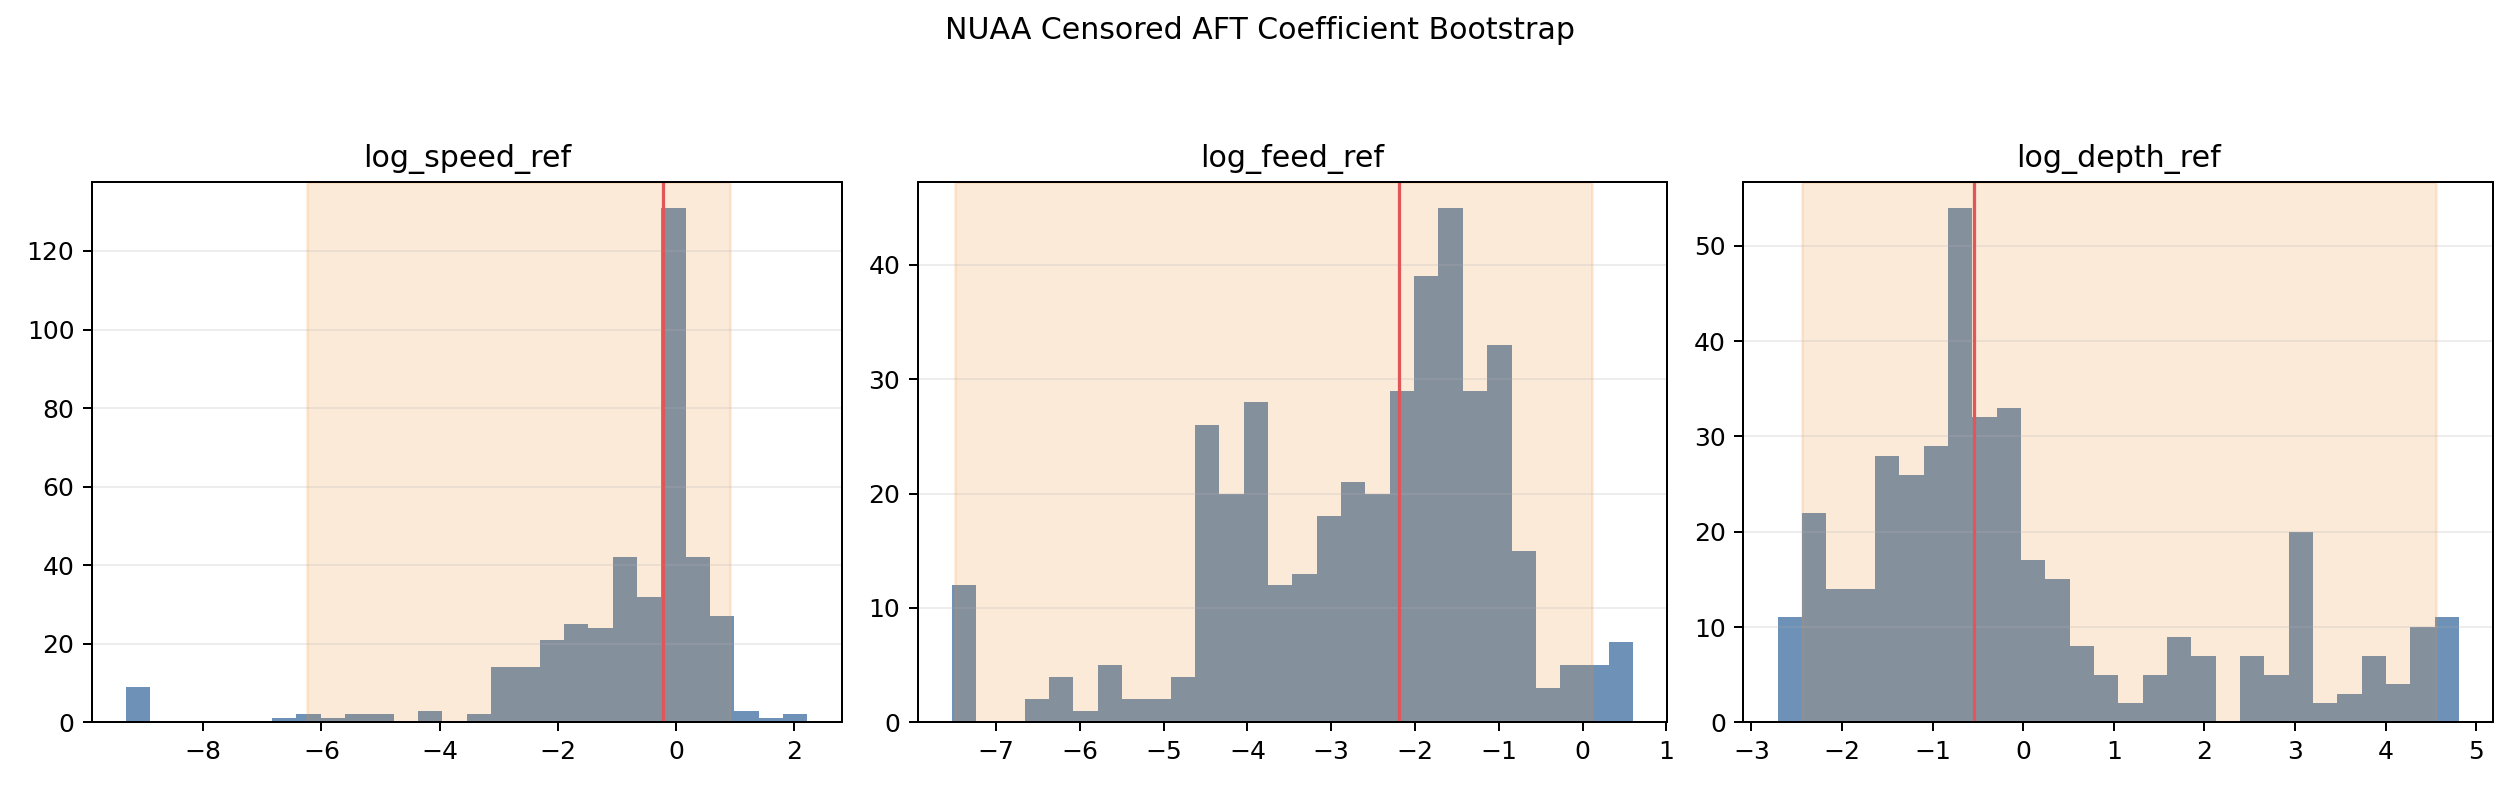
\includegraphics[width=\columnwidth]{nuaa_aft_coefficient_bootstrap.png}
  \caption{NUAA AFT bootstrap uncertainty. Sparse events and censoring make speed and depth effects weakly identified.}
  \label{fig:aft-bootstrap}
\end{figure}

\subsection{ML-inverted and observed life equations}

The Ridge response surface is inverted over a grid of operating scenarios and then compressed into a Taylor-like equation:
\begin{equation}
T_{\min} =
47.52
\left(\frac{n}{1800}\right)^{-10.4924}
\left(\frac{f_z}{0.05}\right)^{-4.6506}
\left(\frac{a_p}{3.0}\right)^{-0.1372},
\label{eq:ridge-life-surface}
\end{equation}
with surrogate log-space \(R^2=0.9800\) over 345 crossing scenarios. The high speed exponent should not be overinterpreted. It warns that the local speed range is narrow and speed is partly confounded with other load effects.

Using only uncensored NUAA threshold crossings gives
\begin{equation}
T_{\min} =
16.78
\left(\frac{n}{1800}\right)^{-12.6655}
\left(\frac{f_z}{0.05}\right)^{-4.1634}
\left(\frac{a_p}{3.0}\right)^{-2.4111},
\label{eq:observed-life}
\end{equation}
with log RMSE \(0.3784\). This observed-life equation is less robust because it discards censored runs, but it independently supports a strong negative feed effect.

\begin{figure}[!htbp]
  \centering
  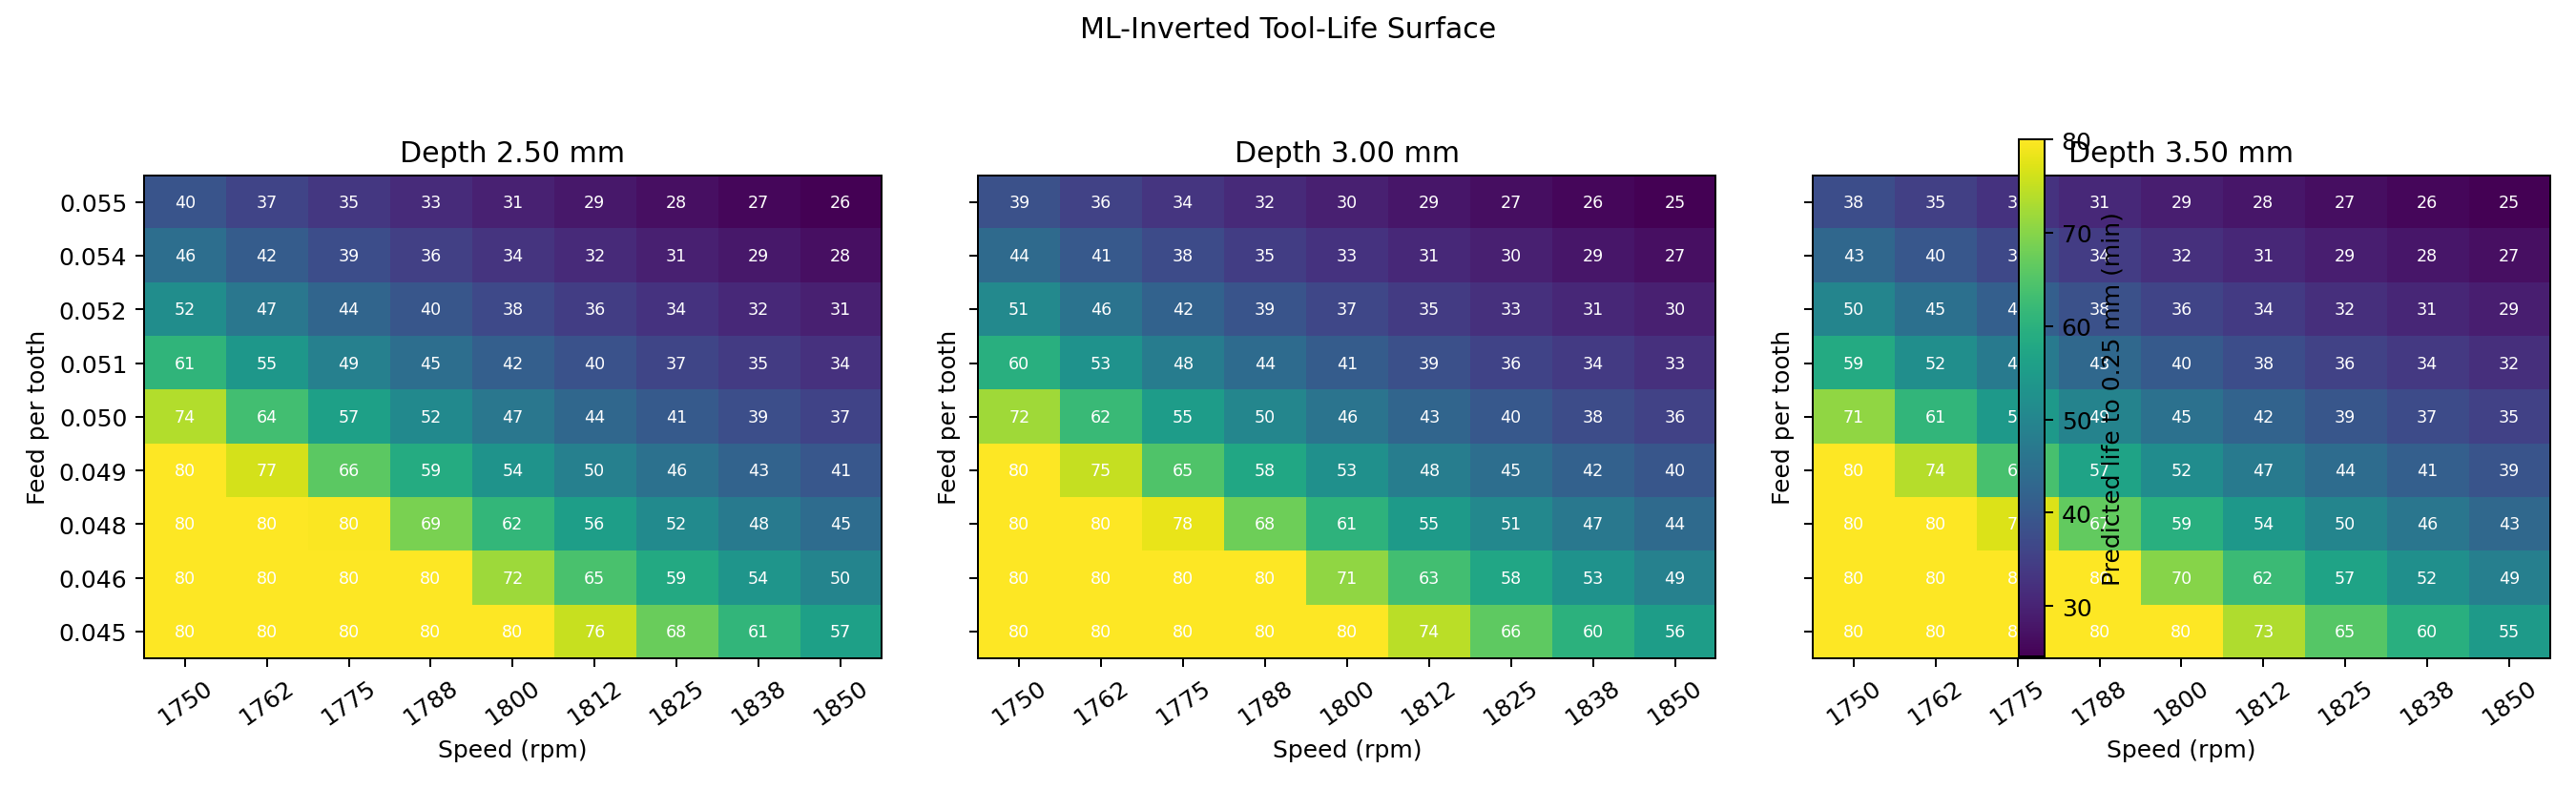
\includegraphics[width=\columnwidth]{ml_life_surface_heatmap.png}
  \caption{ML-inverted NUAA life surface. The surface is useful for scenario ranking but must be interpreted within the training design limits.}
  \label{fig:ml-life-surface}
\end{figure}

\subsection{NASA material-aware life model}

NASA is handled separately because all local NASA threshold labels cross the selected threshold and because material and initial wear carry strong effects. The material-aware AFT model includes feed, depth, material and initial wear.

\begin{table}[!htbp]
  \centering
  \caption{NASA material-aware AFT model summary.}
  \label{tab:nasa-aft}
  \scriptsize
  \begin{tabular}{lrr}
    \toprule
    Term & Coefficient & Mult. effect \\
    \midrule
    Intercept & 4.0880 & 59.6220 \\
    log feed reference & -0.3874 & 0.6788 \\
    log depth reference & -1.1356 & 0.3212 \\
    material: steel & -1.6069 & 0.2005 \\
    initial wear & -3.1201 & 0.0442 \\
    \bottomrule
  \end{tabular}
\end{table}

The NASA AFT fit has event MAE 2.5498, RMSE 3.1544, \(R^2=0.9689\), \(\sigma=0.2459\) and negative log likelihood \(43.6327\). The high \(R^2\) is promising, but it should be interpreted with the small case count and fixed-speed design in mind.

\begin{figure}[!htbp]
  \centering
  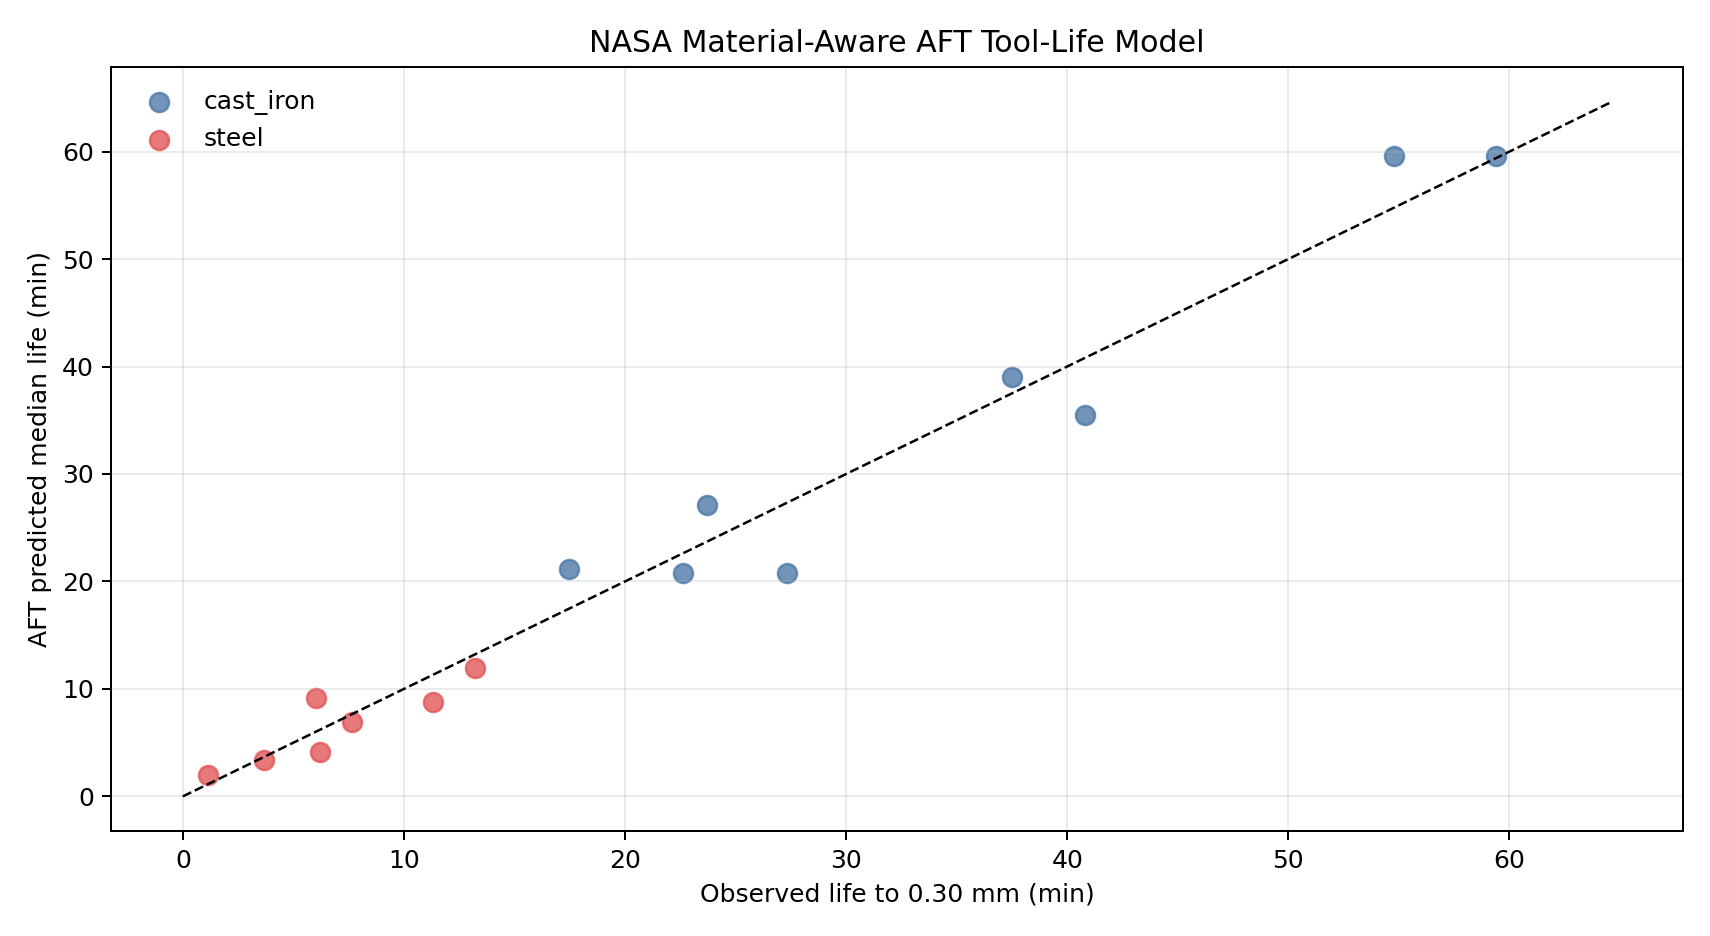
\includegraphics[width=\columnwidth]{nasa_aft_life_model.png}
  \caption{NASA material-aware AFT predictions. Material and initial wear are strong local drivers.}
  \label{fig:nasa-aft}
\end{figure}

\section{Digital-twin interpretation}

The repository includes simulator-oriented model and frontend artifacts. The simulator behavior is driven by the piecewise law and the load-intensity function. It should be understood as a research digital-twin prototype: it maps operating conditions to wear trajectories and life estimates, but its uncertainty bands and known failure modes should remain visible.

\begin{figure}[!htbp]
  \centering
  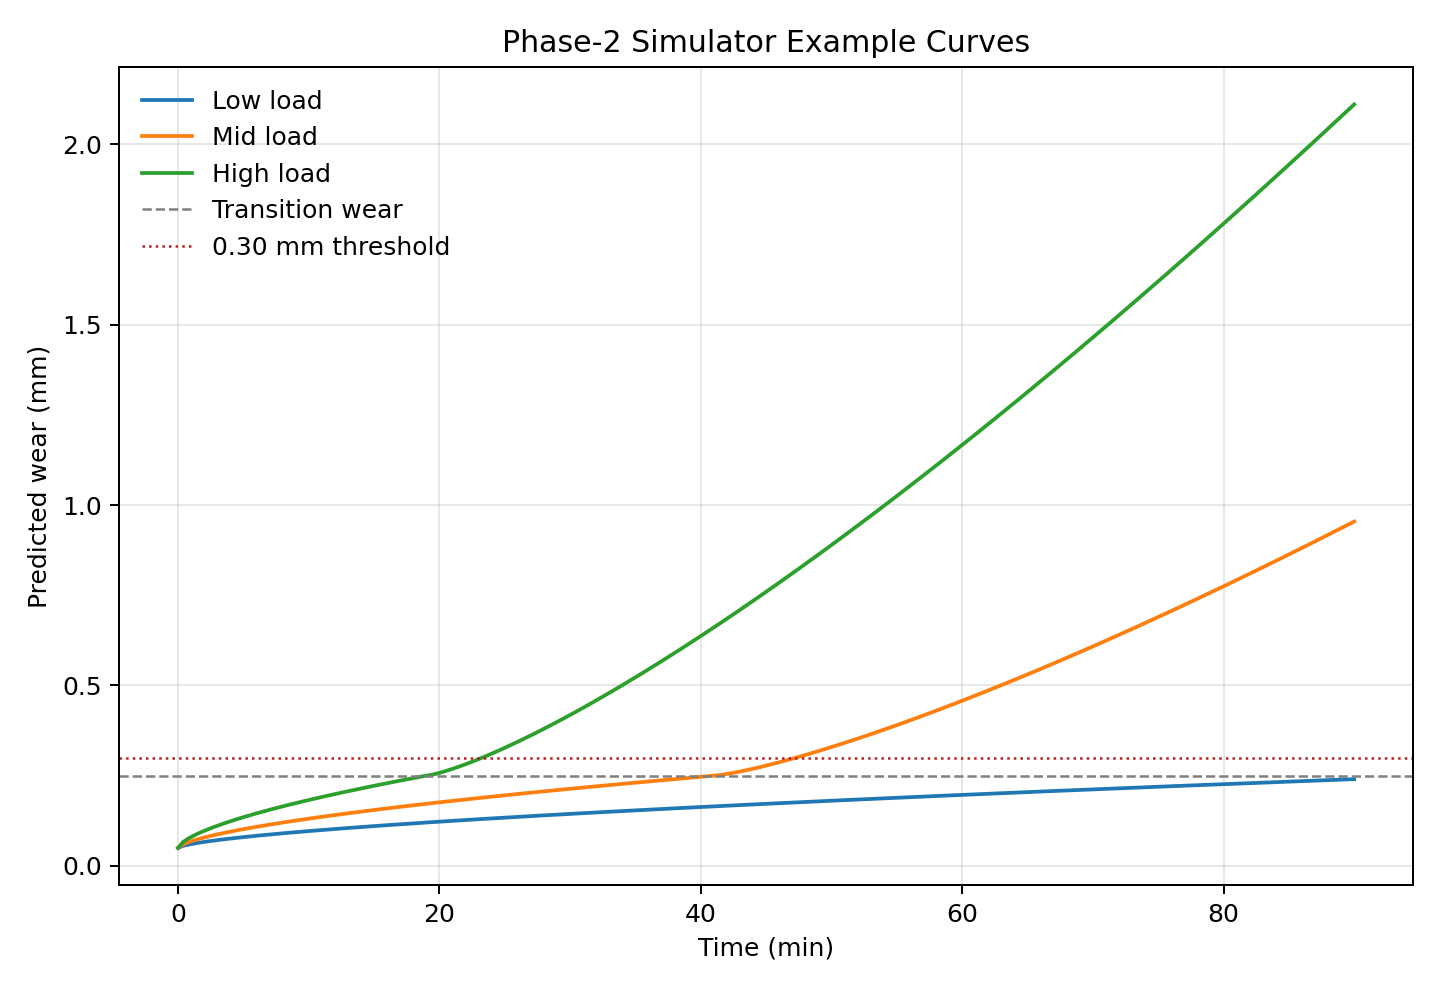
\includegraphics[width=\columnwidth]{simulation_example_curves.png}
  \caption{Example simulated wear curves. The piecewise law produces slow early growth followed by late acceleration.}
  \label{fig:simulation-curves}
\end{figure}

A practical decision workflow follows four steps. First, estimate the expected wear trajectory for the candidate load condition. Second, track sensor health markers, especially vibration and acoustic-emission modal features, for deviation from the expected trajectory. Third, use survival-aware lifetime outputs when threshold crossing is the primary decision. Fourth, treat high-speed exponents and short-window calibrations cautiously because they are less stable in the local data.

The simulator is therefore best used for scenario ranking and explanation. A low-load condition can be compared against a baseline or high-load condition to show how predicted life changes. However, the result should not be presented as a deployment-ready replacement policy until broader full-life milling datasets are ingested and the life model is validated under leave-dataset-out tests.

\section{Limitations and risk}

The main limitations are direct consequences of the available data. The speed exponent is unstable in bootstrap and extracted life equations because the local speed range is narrow and correlated with other design variables. NASA provides strong late-stage and sensor evidence, but its feed units, material labels and fixed-speed design make direct pooling with NUAA unsafe. PHM2010 is valuable for early-regime transfer, but the local use of PHM2010 has only three cutter groups. Gradient Boosting has the best NUAA pointwise wear RMSE but worse event-life MAE after threshold inversion. Per-run scalar calibration from short early windows overcorrects in NUAA holdout tests. Finally, the simulator can look more decisive than the evidence supports unless intervals, limits and dataset provenance are shown.

\begin{table*}[!t]
  \centering
  \caption{Research risk matrix.}
  \label{tab:risk-matrix}
  \footnotesize
  \begin{tabularx}{\textwidth}{p{3.2cm}p{1.7cm}p{3.0cm}Y}
    \toprule
    Risk & Severity & Current evidence & Recommended response \\
    \midrule
    Speed exponent overinterpretation & High & Wide bootstrap interval and large ML-inverted exponent & Report speed sensitivity as provisional and prioritize new experiments with wider speed variation. \\
    Dataset pooling mismatch & High & Different units, sensors and thresholds & Maintain dataset-specific roles and use transfer learning only after unit harmonization. \\
    Calibration overcorrection & Medium & Calibrated RMSE worse than uncalibrated in NUAA & Replace scalar calibration with Bayesian or state-space updating. \\
    Small event count & High & NUAA has 5 events and 4 censored records & Add full-life datasets and keep censoring explicit. \\
    VMD feature overfitting & Medium & Many modal features relative to NASA sample count & Use grouped validation, feature stability and sparse model variants. \\
    Simulator misuse & Medium & Curves can look decisive despite uncertainty & Surface intervals, limits and dataset provenance in the UI. \\
    \bottomrule
  \end{tabularx}
\end{table*}

\section{Conclusions and next work}

The project now contains a coherent research program for milling tool wear and tool-life forecasting. The strongest technical result is not a single machine-learning score. It is the combination of interpretable physics, signal evidence, grouped validation, threshold inversion and censoring-aware life modeling. The piecewise wear law explains why early and late data should not be forced into one undifferentiated fit. VMD and SHAP analyses show which sensor signatures carry wear information. The lifetime extraction pass shows that training a model and inverting it into life is possible, while also showing that the best wear regressor is not necessarily the best life predictor.

The practical conclusions are clear. Feed is the most reliable local load driver. Late-stage material behavior matters. Censoring must be modeled rather than ignored. Short-window scalar calibration is not yet dependable. The current digital twin is ready for research simulation, scenario ranking and explanation, but it needs larger full-life validation before industrial deployment.

The next research step is structured data expansion rather than simply adding more model classes. Each new dataset should be mapped into a common life schema: tool identifier, tool material, coating, cutter geometry, workpiece material, spindle speed or cutting speed, feed per tooth or feed rate, axial and radial depth, wear measurement type, threshold definition, native time base, sensor channels, sampling rate and event/censoring indicator. After ingestion, the piecewise law should be refit, leave-dataset-out validation should be run, scalar calibration should be replaced by a monotonic state-space update, and survival models should combine physics-law covariates with stable VMD summaries.

\begin{table*}[!t]
  \centering
  \caption{Main equations produced by the research.}
  \label{tab:equation-summary}
  \footnotesize
  \begin{tabularx}{\textwidth}{p{3.2cm}Y}
    \toprule
    Model & Equation \\
    \midrule
    Condition intensity &
    \(\phii=(n/1800)^{0.359967}(f_z/0.05)^{3.956013}(a_p/3.0)^{0.688073}\) \\
    Early wear &
    \(\vb(t)=0.018580943\,\phii\,t^{0.64}\) \\
    NUAA censored AFT &
    \(T_{\min}=24.93(n/1800)^{-0.0187}(f_z/0.05)^{-1.7662}(a_p/3.0)^{-0.3768}\) \\
    Ridge-inverted life surface &
    \(T_{\min}=47.52(n/1800)^{-10.4924}(f_z/0.05)^{-4.6506}(a_p/3.0)^{-0.1372}\) \\
    Observed-life equation &
    \(T_{\min}=16.78(n/1800)^{-12.6655}(f_z/0.05)^{-4.1634}(a_p/3.0)^{-2.4111}\) \\
    \bottomrule
  \end{tabularx}
\end{table*}

\clearpage
\section*{Acknowledgements}

The authors acknowledge the Department of Mechanical Engineering, BITS Pilani, and the public milling datasets used for this research workflow.

\section*{References}

\footnotesize
\setlength{\parindent}{0pt}
\setlength{\parskip}{0.35em}

Dragomiretskiy, K. and Zosso, D. (2014) `Variational mode decomposition', \textit{IEEE Transactions on Signal Processing}, 62(3), pp. 531--544.

Jain, A.K. and Lad, B.K. (2020) `Prognosticating RULs while exploiting the future characteristics of operating profiles', \textit{Reliability Engineering and System Safety}, 202, 107031.

Katzman, J.L., Shaham, U., Cloninger, A., Bates, J., Jiang, T. and Kluger, Y. (2018) `DeepSurv: personalized treatment recommender system using a Cox proportional hazards deep neural network', \textit{BMC Medical Research Methodology}, 18(1), 24.

Li, X., Lim, B.S., Zhou, J.H., Huang, S., Phua, S.J., Shaw, K.C. and Er, M.J. (2010) `Fuzzy neural network modelling for tool wear estimation in dry milling operation', in \textit{Proceedings of the Annual Conference of the Prognostics and Health Management Society}.

NASA Prognostics Center of Excellence (n.d.) \textit{Milling Data Set}. NASA PCoE data repository.

Raissi, M., Perdikaris, P. and Karniadakis, G.E. (2019) `Physics-informed neural networks: a deep learning framework for solving forward and inverse problems involving nonlinear partial differential equations', \textit{Journal of Computational Physics}, 378, pp. 686--707.

Sankararaman, S. and Goebel, K. (2015) `Why is the remaining useful life prediction uncertain?', in \textit{Proceedings of the Annual Conference of the Prognostics and Health Management Society}, pp. 337--349.

Sun, H., Zhang, J., Mo, R. and Zhang, X. (2023) `In-process tool condition forecasting based on a deep learning method', \textit{Sensors}, 23(7), 3527.

UniWear / NUAA Consortium (n.d.) \textit{UniWear orthogonal milling wear records}. Nanjing University of Aeronautics and Astronautics. Local dataset documentation.

Wang, J., Xie, J., Zhao, R., Zhang, L. and Duan, L. (2017) `Multisensory fusion based virtual tool wear sensing for ubiquitous manufacturing', \textit{Robotics and Computer-Integrated Manufacturing}, 45, pp. 47--58.

Zhao, R., Yan, R., Chen, Z., Mao, K., Wang, P. and Gao, R.X. (2019) `Deep learning and its applications to machine health monitoring', \textit{Mechanical Systems and Signal Processing}, 115, pp. 213--237.

\end{document}
